         \chapter{Equations and inequalities}
    \setcounter{figure}{1}
    \setcounter{subfigure}{1}
    \label{108b030756318cdc732e3f8c9c583cfb}
%        
%          \section{ Strategy for solving equations}
%     \nopagebreak
%             \label{m39250} $ \hspace{-5pt}\begin{array}{cccccccccccc}   \end{array} $ \hspace{2 pt}\raisebox{-5 pt}{
\includegraphics[width=0.5cm]{col11306.imgs/summary_www.png}} {(section shortcode: MG10067 )} \par 
%     
%     
%     
%     
%     
%     
%   
%     \label{m39250*cid2}
%             \subsection{ Strategy for Solving Equations}
%             \nopagebreak
%             
%       
%       \label{m39250*id143934}This chapter is all about solving different types of equations for one or two variables. In general, we want to get the unknown variable alone on the left hand side of the equation with all the constants on the right hand side of the equation. For example, in the equation $x-1=0$\hspace{1ex}, we want to be able to write the equation as $x=1$.\par 
%       \label{m39250*id144309}As we saw in rearranging equations\footnote{\raggedright{}"Review of Past Work": Section Rearranging Equations <http://http://cnx.org/content/m31330/latest/\#cid10>}, an equation is like a set of weighing scales that must always be balanced. When we solve equations, we need to keep in mind that what is done to one side must be done to the other.\par 
%       \label{m39250*uid1}
%             \subsubsection{ Method: Rearranging Equations}
%             \nopagebreak
%             
%         
%         \label{m39250*id144329}You can add, subtract, multiply or divide both sides of an equation by any number you want, as long as you always do it to both sides.\par 
%         \label{m39250*id144333}For example, in the equation $x+5-1=-6$\hspace{1ex}, we want to get $x$ alone on the left hand side of the equation. This means we need to subtract 5 and add 1 on the left hand side. However, because we need to keep the equation balanced, we also need to subtract 5 and add 1 on the right hand side.\par 
%         \label{m39250*id144370}\nopagebreak\noindent{}
%           
%     \begin{equation}
%     \begin{array}{ccc}\hfill x+5-1& =& -6\hfill \\ \hfill x+5-5-1+1& =& -6-5+1\hfill \\ \hfill x+0+0& =& -11+1\hfill \\ \hfill x& =& -10\hfill \end{array}\tag{9.1}
%       \end{equation}
%     
%         
%         \label{m39250*id144503}In another example, $\frac{2}{3}x=8$, we must divide by 2 and multiply by 3 on the left hand side in order to get $x$ alone. However, in order to keep the equation balanced, we must also divide by 2 and multiply by 3 on the right hand side.\par 
%         \label{m39250*id144535}\nopagebreak\noindent{}
%           
%     \begin{equation}
%     \begin{array}{ccc}\hfill \frac{2}{3}x& =& 8\hfill \\ \hfill \frac{2}{3}xÃ\ensuremath{\cdot}2Ã---3& =& 8Ã\ensuremath{\cdot}2Ã---3\hfill \\ \hfill \frac{2}{2}Ã---\frac{3}{3}Ã---x& =& \frac{8Ã---3}{2}\hfill \\ \hfill 1Ã---1Ã---x& =& 12\hfill \\ \hfill x& =& 12\hfill \end{array}\tag{9.2}
%       \end{equation}
%     
%         
%         \label{m39250*id144692}These are the basic rules to apply when simplifying any equation. In most cases, these rules have to be applied more than once, before we have the unknown variable on the left hand side of the equation.\par 
%         
% \label{m39250*notfhsst!!!underscore!!!id254}
% \begin{tabular}{cc}
% 	   \hspace*{-50pt}\raisebox{-8 mm}{ 
\includegraphics[width=0.5in]{col11306.imgs/pstip2.png}  }& 
% 
% 	\begin{minipage}{0.85\textwidth}
% 	\begin{note}
%       {tip: }The following must also be kept in mind:
%         \label{m39250*id144706}\begin{enumerate}[noitemsep, label=\textbf{\arabic*}. ] 
%             \label{m39250*uid2}\item Division by 0 is undefined.
% \label{m39250*uid3}\item If $\frac{x}{y}=0$, then $x=0$ and $y\^{a}‰~0$, because division by 0 is
% undefined.
% \end{enumerate}
%         
% 
% 	\end{note}
% 	\end{minipage}
% 	\end{tabular}
% 	\par
%       
% \label{m39250*id144697}We are now ready to solve some equations!\par 
% \label{m39250*secfhsst!!!underscore!!!id263}
%             \subsubsection{ Investigation : 4 = 3 ??}
%             \nopagebreak
%             
%         \label{m39250*id144787}In the following,
% identify what is wrong.\par 
%         \label{m39250*id144793}\nopagebreak\noindent{}
%     \begin{equation}
%     \begin{array}{ccc}\hfill x& =& 2\hfill \\ \hfill 4x-8& =& 3x-6\hfill \\ \hfill 4\left(x-2\right)& =& 3\left(x-2\right)\hfill \\ \hfill \frac{4\left(x-2\right)}{\left(x-2\right)}& =& \frac{3\left(x-2\right)}{\left(x-2\right)}\hfill \\ \hfill 4& =& 3\hfill \end{array}\tag{9.3}
%       \end{equation}
%     
%         
%         
% 
%       
%     
% \label{m39250**end}
         \section{ Solving linear equations}
    \nopagebreak
            \label{m39241} $ \hspace{-5pt}\begin{array}{cccccccccccc}   
\includegraphics[width=0.75cm]{col11306.imgs/summary_fullmarks.png} &   
\includegraphics[width=0.75cm]{col11306.imgs/summary_video.png} &   \end{array} $ \hspace{2 pt}\raisebox{-5 pt}{} {(section shortcode: MG10068 )} \par 
% \label{m39241*cid3}
%             \subsection{ Equations and inequalities: Solving linear equations}
%             \nopagebreak
%             
\label{m39241*id145155}The simplest equation to solve is a linear equation. A linear equation is an
equation where the power of the variable(letter, e.g. $x$) is 1(one). The
following are examples of linear equations.\par 
      \label{m39241*id145168}\nopagebreak\noindent{}
        
    \begin{equation}
    \begin{array}{ccc}\hfill 2x+2& =& 1\hfill \\ \hfill \frac{2-x}{3x+1}& =& 2\hfill \\ \hfill \frac{4}{3}x-6& =& 7x+2\hfill \end{array}\tag{9.4}
      \end{equation}
      \label{m39241*id145267}In this section, we will learn how to find the value of the variable that makes
both sides of the linear equation true. For example, what value of $x$ makes
both sides of the very simple equation, $x+1=1$ true.\par 
      \label{m39241*id145297}Since the definition of a linear equation is that if the variable has a highest power of one (1), there is
at most \textsl{one solution} or \textsl{root} for the equation.\par 
      \label{m39241*id145312}This section relies on all the methods we have already discussed: multiplying
out expressions, grouping terms and factorisation. Make sure that you are
comfortable with these methods, before trying out the work in the rest of this
chapter.\par 
      \label{m39241*id145317}\nopagebreak\noindent{}
    \begin{equation}
    \begin{array}{cccc}\hfill 2x+2& =& 1\hfill & \\ \hfill 2x& =& 1-2\hfill & \left(\mathrm{like\; terms\; together}\right)\hfill & \\ \hfill 2x& =& -1\hfill & \left(\mathrm{simplified\; as\; much\; as\; possible}\right)\hfill & \end{array}\tag{9.5}
      \end{equation}
      \label{m39241*id145430}Now we see that $2x=-1$. This means if we divide both sides by 2, we will get:\par 
      \label{m39241*id145453}\nopagebreak\noindent{}
        
    \begin{equation}
    x=-\frac{1}{2}\tag{9.6}
      \end{equation}
      \label{m39241*id145475}If we substitute $x=-\frac{1}{2}$, back into the original equation, we get:\par 
      \label{m39241*id145500}\nopagebreak\noindent{}
    \begin{equation}
    \begin{array}{ccc}\hfill \mathrm{LHS}& =& 2x+2\hfill \\ & =& 2\left(-\frac{1}{2}\right)+2\hfill \\ & =& -1+2\hfill \\ & =& 1\hfill \\ \hfill \mathrm{and}\\ \hfill \mathrm{RHS}& =& 1\hfill \end{array}\tag{9.7}
      \end{equation}
      \label{m39241*id145603}That is all that there is to solving linear equations.\par 
\label{m39241*notfhsst!!!underscore!!!id622}
\begin{tabular}{cc}
	   \hspace*{-50pt}\raisebox{-8 mm}{ 
\includegraphics[width=0.5in]{col11306.imgs/pstip2.png}  }& 
	\begin{minipage}{0.85\textwidth}
	\begin{note}
      {tip: }When you have found the solution to an equation,
substitute the solution into the original equation, to check your answer.
	\end{note}
	\end{minipage}
	\end{tabular}
	\par
      \label{m39241*uid4}
            \subsubsubsection{ Method: Solving Linear Equations}
            \nopagebreak
            \label{m39241*id145627}The general steps to solve linear equations are:\par 
        \label{m39241*id145635}\begin{enumerate}[noitemsep, label=\textbf{\arabic*}. ] 
            \label{m39241*uid5}\item  Expand (Remove) all brackets that are in the equation.
\label{m39241*uid6}\item  "Move" all terms with the variable to the left hand side of the equation, and
all constant terms (the numbers) to the right hand side of the equals sign.
Bearing in mind that the sign of the terms will change from ($+$) to ($-$) or vice
versa, as they "cross over" the equals sign.
\label{m39241*uid7}\item Group all like terms together and simplify as much as possible.
\label{m39241*uid8}\item  If necessary factorise.
\label{m39241*uid9}\item  Find the solution and write down the answer(s).
\label{m39241*uid10}\item Substitute solution into \textbf{original} equation to check answer.
\end{enumerate}
\label{m39241*eip-126}
    \setcounter{subfigure}{0}
	\begin{figure}[H] % horizontal\label{m39241*equations-1}
    \textnormal{Khan academy video on equations - 1}\vspace{.1in} \nopagebreak
  \label{m39241*yt-media1}\label{m39241*yt-video1}
            \raisebox{-5 pt}{ 
\includegraphics[width=0.5cm]{col11306.imgs/summary_www.png}} { (Video:  MG10069 )}
      \vspace{2pt}
    \vspace{.1in}
 \end{figure}       \par \label{m39241*secfhsst!!!underscore!!!id646}\vspace{.5cm} 
      \noindent
      \hspace*{-30pt}
\includegraphics[width=0.5in]{col11306.imgs/pspencil2.png}   \raisebox{25mm}{   
      \begin{mdframed}[linewidth=4, leftmargin=40, rightmargin=40]  
      \begin{exercise}
    \noindent\textbf{Exercise 9.1:  Solving Linear Equations }
        \label{m39241*probfhsst!!!underscore!!!id647}
        \label{m39241*id145728}Solve for $x$: $4-x=4$ \par 
        \vspace{5pt}
        \label{m39241*solfhsst!!!underscore!!!id650}\noindent\textbf{Solution to Exercise } \label{m39241*listfhsst!!!underscore!!!id650}\begin{enumerate}[noitemsep, label=\textbf{Step} \textbf{\arabic*}. ] 
            \leftskip=20pt\rightskip=\leftskip\item  
        \label{m39241*id145775}We are given $4-x=4$ and are required to solve for $x$.\par 
        \item  
        \label{m39241*id145807}Since there are no brackets, we can start with rearranging and then grouping like terms.\par 
        \item  
        \label{m39241*id145815}\nopagebreak\noindent{}
    \begin{equation}
    \begin{array}{cccc}\hfill 4-x& =& 4\hfill & \\ \hfill -x& =& 4-4\hfill & \left(\mathrm{Rearrange}\right)\hfill \\ \hfill -x& =& 0\hfill & \left(\mathrm{group\; like\; terms}\right)\hfill \\ \hfill \^{a}ˆ´x& =& 0\hfill & \end{array}\tag{9.8}
      \end{equation}
        \item  
        \label{m39241*id146022}Substitute solution into original equation:\par 
        \label{m39241*id146026}\nopagebreak\noindent{}
    \begin{equation}
    \begin{array}{ccc}\hfill 4-0& =& 4\hfill \\ \hfill 4& =& 4\hfill \end{array}\tag{9.9}
      \end{equation}
        \label{m39241*id146060}Since both sides are equal, the answer is correct.\par 
        \item  
        \label{m39241*id146070}The solution of $4-x=4$ is $x=0$.
 \par 
        \end{enumerate}
    \end{exercise}
    \end{mdframed}
    }
    \noindent
\label{m39241*secfhsst!!!underscore!!!id822}\vspace{.5cm} 
      \noindent
      \hspace*{-30pt}
\includegraphics[width=0.5in]{col11306.imgs/pspencil2.png}   \raisebox{25mm}{   
      \begin{mdframed}[linewidth=4, leftmargin=40, rightmargin=40]  
      \begin{exercise}
    \noindent\textbf{Exercise 9.2:  Solving Linear Equations }
        \label{m39241*probfhsst!!!underscore!!!id823}
        \label{m39241*id146127}Solve for $x$: $4\left(2x-9\right)-4x=4-6x$ \par 
        \vspace{5pt}
        \label{m39241*solfhsst!!!underscore!!!id826}\noindent\textbf{Solution to Exercise } \label{m39241*listfhsst!!!underscore!!!id826}\begin{enumerate}[noitemsep, label=\textbf{Step} \textbf{\arabic*}. ] 
            \leftskip=20pt\rightskip=\leftskip\item  
        \label{m39241*id146196}We are given $4\left(2x-9\right)-4x=4-6x$ and are required to solve for $x$.\par 
        \item  
        \label{m39241*id146249}We start with expanding the brackets, then rearranging, then grouping like terms and then
simplifying.\par 
        \item  
        \label{m39241*id146257}\nopagebreak\noindent{}
    \begin{equation}
    \begin{array}{cccc}\hfill 4\left(2x-9\right)-4x& =& 4-6x\hfill & \\ \hfill 8x-36-4x& =& 4-6x\hfill & \left(\mathrm{expand\; the\; brackets}\right)\hfill \\ \hfill 8x-4x+6x& =& 4+36\hfill & \left(\mathrm{Rearrange}\right)\hfill \\ \hfill \left(8x-4x+6x\right)& =& \left(4+36\right)\hfill & \left(\mathrm{group\; like\; terms}\right)\hfill \\ \hfill 10x& =& 40\hfill & \left(\mathrm{simplify\; grouped\; terms}\right)\hfill \\ \hfill \frac{10}{10}x& =& \frac{40}{10}\hfill & \left(\mathrm{divide\; both\; sides\; by}\phantom{\rule{2pt}{0ex}}10\right)\hfill \\ \hfill x& =& 4\hfill & \end{array}\tag{9.10}
      \end{equation}
        \item  
        \label{m39241*id146645}Substitute solution into original equation:\par 
        \label{m39241*id146649}\nopagebreak\noindent{}
          
    \begin{equation}
    \begin{array}{ccc}\hfill 4\left(2\left(4\right)-9\right)-4\left(4\right)& =& 4-6\left(4\right)\hfill \\ \hfill 4\left(8-9\right)-16& =& 4-24\hfill \\ \hfill 4\left(-1\right)-16& =& -20\hfill \\ \hfill -4-16& =& -20\hfill \\ \hfill -20& =& -20\hfill \end{array}\tag{9.11}
      \end{equation}
        \label{m39241*id146831}Since both sides are equal to $-20$, the answer is correct.\par 
        \item  
        \label{m39241*id146854}The solution of $4\left(2x-9\right)-4x=4-6x$ is $x=4$.
 \par 
        \end{enumerate}
    \end{exercise}
    \end{mdframed}
    }
    \noindent
\label{m39241*secfhsst!!!underscore!!!id1189}\vspace{.5cm} 
      \noindent
      \hspace*{-30pt}
\includegraphics[width=0.5in]{col11306.imgs/pspencil2.png}   \raisebox{25mm}{   
      \begin{mdframed}[linewidth=4, leftmargin=40, rightmargin=40]  
      \begin{exercise}
    \noindent\textbf{Exercise 9.3:  Solving Linear Equations }
        \label{m39241*probfhsst!!!underscore!!!id1190}
        \label{m39241*id146935}Solve for $x$: $\frac{2-x}{3x+1}=2$ \par 
        \vspace{5pt}
        \label{m39241*solfhsst!!!underscore!!!id1193}\noindent\textbf{Solution to Exercise } \label{m39241*listfhsst!!!underscore!!!id1193}\begin{enumerate}[noitemsep, label=\textbf{Step} \textbf{\arabic*}. ] 
            \leftskip=20pt\rightskip=\leftskip\item  
        \label{m39241*id146999}We are given $\frac{2-x}{3x+1}=2$ and are required to solve for $x$.\par 
        \item  
        \label{m39241*id147046}Since there is a denominator of ($3x+1$), we can start by multiplying both sides
of the equation by ($3x+1$). But because division by 0 is not permissible, there
is a restriction on a value for x. ($x\^{a}‰~\frac{-1}{3}$)\par 
        \item  
        \label{m39241*id147077}\nopagebreak\noindent{}
    \begin{equation}
    \begin{array}{cccc}\hfill \frac{2-x}{3x+1}& =& 2\hfill & \\ \hfill \left(2-x\right)& =& 2\left(3x+1\right)\hfill & \\ \hfill 2-x& =& 6x+2\hfill & \left(\mathrm{expand\; brackets}\right)\hfill \\ \hfill -x-6x& =& 2-2\hfill & \left(\mathrm{rearrange}\right)\hfill \\ \hfill -7x& =& 0\hfill & \left(\mathrm{simplify\; grouped\; terms}\right)\hfill \\ \hfill x& =& 0Ã\ensuremath{\cdot}\left(-7\right)\hfill & \\ \hfill \^{a}ˆ´\; \; \phantom{\rule{2.em}{0ex}}x& =& 0\hfill & \left(\mathrm{zero\; divided\; by\; any\; number\; is}\phantom{\rule{3pt}{0ex}}0\right)\hfill \end{array}\tag{9.12}
      \end{equation}
        \item  
        \label{m39241*id147437}Substitute solution into original equation:\par 
        \label{m39241*id147441}\nopagebreak\noindent{}
          
    \begin{equation}
    \begin{array}{ccc}\hfill \frac{2-\left(0\right)}{3\left(0\right)+1}& =& 2\hfill \\ \hfill \frac{2}{1}& =& 2\hfill \end{array}\tag{9.13}
      \end{equation}
        \label{m39241*id147513}Since both sides are equal to 2, the answer is correct.\par 
        \item  
        \label{m39241*id147525}The solution of $\frac{2-x}{3x+1}=2$ is $x=0$.
 \par 
        \end{enumerate}
    \end{exercise}
    \end{mdframed}
    }
    \noindent
\label{m39241*secfhsst!!!underscore!!!id1472}\vspace{.5cm} 
      \noindent
      \hspace*{-30pt}
\includegraphics[width=0.5in]{col11306.imgs/pspencil2.png}   \raisebox{25mm}{   
      \begin{mdframed}[linewidth=4, leftmargin=40, rightmargin=40]  
      \begin{exercise}
    \noindent\textbf{Exercise 9.4:  Solving Linear Equations }
        \label{m39241*probfhsst!!!underscore!!!id1473}
        \label{m39241*id147599}Solve for $x$: $\frac{4}{3}x-6=7x+2$ \par 
        \vspace{5pt}
        \label{m39241*solfhsst!!!underscore!!!id1476}\noindent\textbf{Solution to Exercise } \label{m39241*listfhsst!!!underscore!!!id1476}\begin{enumerate}[noitemsep, label=\textbf{Step} \textbf{\arabic*}. ] 
            \leftskip=20pt\rightskip=\leftskip\item  
        \label{m39241*id147662}We are given $\frac{4}{3}x-6=7x+2$ and are required to solve for $x$.\par 
        \item  
        \label{m39241*id147710}We start with multiplying each of the terms in the equation by 3, then
grouping like terms and then simplifying.\par 
        \item  
        \label{m39241*id147718}\nopagebreak\noindent{}
    \begin{equation}
    \begin{array}{cccc}\hfill \frac{4}{3}x-6& =& 7x+2\hfill & \\ \hfill 4x-18& =& 21x+6\hfill & \left(\mathrm{each\; term\; is\; multiplied\; by}\phantom{\rule{3pt}{0ex}}3\right)\hfill \\ \hfill 4x-21x& =& 6+18\hfill & \left(\mathrm{rearrange}\right)\hfill \\ \hfill -17x& =& 24\hfill & \left(\mathrm{simplify\; grouped\; terms}\right)\hfill \\ \hfill \frac{-17}{-17}x& =& \frac{24}{-17}\hfill & \left(\mathrm{divide\; both\; sides\; by}\phantom{\rule{2pt}{0ex}}-17\right)\hfill \\ \hfill x& =& \frac{-24}{17}\hfill & \end{array}\tag{9.14}
      \end{equation}
        \item  
        \label{m39241*id148040}Substitute solution into original equation:\par 
        \label{m39241*id148044}\nopagebreak\noindent{}
          
    \begin{equation}
    \begin{array}{ccc}\hfill \frac{4}{3}Ã---\frac{-24}{17}-6& =& 7Ã---\frac{-24}{17}+2\hfill \\ \hfill \frac{4Ã---\left(-8\right)}{\left(17\right)}-6& =& \frac{7Ã---\left(-24\right)}{17}+2\hfill \\ \hfill \frac{\left(-32\right)}{17}-6& =& \frac{-168}{17}+2\hfill \\ \hfill \frac{-32-102}{17}& =& \frac{\left(-168\right)+34}{17}\hfill \\ \hfill \frac{-134}{17}& =& \frac{-134}{17}\hfill \end{array}\tag{9.15}
      \end{equation}
        \label{m39241*id148292}Since both sides are equal to $\frac{-134}{17}$, the answer is correct.\par 
        \item  
        \label{m39241*id148321}The solution of $\frac{4}{3}x-6=7x+2$ is,\ensuremath{\hat{A}}~\ensuremath{\hat{A}}~\ensuremath{\hat{A}}~$x=\frac{-24}{17}$.
 \par 
        \end{enumerate}
    \end{exercise}
    \end{mdframed}
    }
    \noindent
\label{m39241*secfhsst!!!underscore!!!id1862}
            \subsubsection{ Exercise: Solving Linear Equations }
            \nopagebreak
        \label{m39241*id148396}\begin{enumerate}[noitemsep, label=\textbf{\arabic*}. ] 
            \label{m39241*uid11}\item Solve for $y$: $2y-3=7$\hspace{1ex}        
\label{m39241*uid12}\item Solve for $y$: $-3y=0$\hspace{1ex}        
\label{m39241*uid13}\item Solve for $y$: $4y=16$\hspace{1ex}        
\label{m39241*uid14}\item Solve for $y$: $12y+0=144$\hspace{1ex}        
\label{m39241*uid15}\item Solve for $y$: $7+5y=62$\hspace{1ex}        
\label{m39241*uid16}\item Solve for $x$: $55=5x+\frac{3}{4}$\hspace{1ex}        
\label{m39241*uid17}\item Solve for $x$: $5x=3x+45$\hspace{1ex}        
\label{m39241*uid18}\item Solve for $x$: $23x-12=6+2x$\hspace{1ex}        
\label{m39241*uid19}\item Solve for $x$: $12-6x+34x=2x-24-64$\hspace{1ex}        
\label{m39241*uid20}\item Solve for $x$: $6x+3x=4-5\left(2x-3\right)$\hspace{1ex}        
\label{m39241*uid21}\item Solve for $p$: $18-2p=p+9$\hspace{1ex}        
\label{m39241*uid22}\item Solve for $p$: $\frac{4}{p}=\frac{16}{24}$\hspace{1ex}        
\label{m39241*uid23}\item Solve for $p$: $\frac{4}{1}=\frac{p}{2}$\hspace{1ex}        
\label{m39241*uid24}\item Solve for $p$: $-\left(-16-p\right)=13p-1$\hspace{1ex}        
\label{m39241*uid25}\item Solve for $p$: $6p-2+2p=-2+4p+8$\hspace{1ex}        
\label{m39241*uid26}\item Solve for $f$: $3f-10=10$\hspace{1ex}        
\label{m39241*uid27}\item Solve for $f$: $3f+16=4f-10$\hspace{1ex}        
\label{m39241*uid28}\item Solve for $f$: $10f+5+0=-2f+-3f+80$\hspace{1ex}        
\label{m39241*uid29}\item Solve for $f$: $8\left(f-4\right)=5\left(f-4\right)$\hspace{1ex}        
\label{m39241*uid30}\item Solve for $f$: $6=6\left(f+7\right)+5f$\hspace{1ex}        
\end{enumerate}
\label{m39241**end}
\par \raisebox{-5 pt}{
\includegraphics[width=0.5cm]{col11306.imgs/summary_www.png}} Find the answers with the shortcodes:
 \par \begin{tabular}[h]{cccccc}
 (1.) lcR  &  (2.) lcR  &  (3.) lcR  &  (4.) lcR  &  (5.) lcR  &  (6.) lcn  &  (7.) lcn  &  (8.) lcn  &  (9.) lcn  &  (10.) lcn  &  (11.) lcQ  &  (12.) lcQ  &  (13.) lcQ  &  (14.) lcQ  &  (15.) lcQ  &  (16.) lcU  &  (17.) lcU  &  (18.) lcU  &  (19.) lcU  &  (20.) lcU  & \end{tabular}
         \section{ Solving quadratic equations}
    \nopagebreak
            \label{m39247} $ \hspace{-5pt}\begin{array}{cccccccccccc}   
\includegraphics[width=0.75cm]{col11306.imgs/summary_fullmarks.png} &   
\includegraphics[width=0.75cm]{col11306.imgs/summary_video.png} &   \end{array} $ \hspace{2 pt}\raisebox{-5 pt}{} {(section shortcode: MG10070 )} \par 
% \label{m39247*cid4}
%             \subsection{ Equations and inequalities: Solving quadratic equations}
%             \nopagebreak
%             
\label{m39247*id149356}A quadratic equation is an equation where the power of the variable is at most
2. The following are examples of quadratic equations.\par 
      \label{m39247*id149360}\nopagebreak\noindent{}
        
    \begin{equation}
    \begin{array}{ccc}\hfill 2{x}^{2}+2x& =& 1\hfill \\ \hfill \frac{2-x}{3x+1}& =& 2x\hfill \\ \hfill \frac{4}{3}x-6& =& 7{x}^{2}+2\hfill \end{array}\tag{9.16}
      \end{equation}
      \label{m39247*id149478}Quadratic equations differ from linear equations by the fact that a linear
equation only has one solution, while a quadratic equation has \textsl{at most}
two solutions. However, there are some special situations when a quadratic equation only
has one solution.\par 
      \label{m39247*id149489}We solve quadratic equations by factorisation, that is writing the quadratic as
a product of two expressions in brackets. For example, we know that:\par 
      \label{m39247*id149493}\nopagebreak\noindent{}
        
    \begin{equation}
    \left(x+1\right)\left(2x-3\right)=2{x}^{2}-x-3.\tag{9.17}
      \end{equation}
      \label{m39247*id149552}In order to solve:\par 
      \label{m39247*id149557}\nopagebreak\noindent{}
        
    \begin{equation}
    2{x}^{2}-x-3=0\tag{9.18}
      \end{equation}
      \label{m39247*id149590}we need to be able to write $2{x}^{2}-x-3$ as $\left(x+1\right)\left(2x-3\right)$, which we already know
% how to do. The reason for equating to zero and factoring is that if we attempt to solve it in a 'normal' way, we may miss one of the solutions. On the other hand, if we have the (non-linear) equation $f\left(x\right)g\left(x\right)=0$, for some functions $f$ and $g$, we know that the solution is $f\left(x\right)=0$ OR $g\left(x\right)=0$, which allows us to find BOTH solutions (or know that there is only one solution if it turns out that $f=g$).\par 
% \label{m39247*secfhsst!!!underscore!!!id2031}
%             \subsubsection{  Investigation : Factorising a Quadratic }
%             \nopagebreak
%             
%       \label{m39247*id149660}Factorise the following
% quadratic expressions:\par 
%       \label{m39247*id149666}\begin{enumerate}[noitemsep, label=\textbf{\arabic*}. ] 
%             \label{m39247*uid31}\item 
%           $x+{x}^{2}$
%         \label{m39247*uid32}\item 
%           ${x}^{2}+1+2x$
%         \label{m39247*uid33}\item 
%           ${x}^{2}-4x+5$
%         \label{m39247*uid34}\item 
%           $16{x}^{2}-9$
%         \label{m39247*uid35}\item 
%           $4{x}^{2}+4x+1$
%         \end{enumerate}
%         
%       
% 
%       \label{m39247*id149848}Being able to factorise a quadratic means that you are one step away from
% solving a quadratic equation. For example, ${x}^{2}-3x-2=0$ can be written as
% $\left(x-1\right)\left(x-2\right)=0$. This means that both $x-1=0$ and $x-2=0$, which gives $x=1$ and
% $x=2$ as the two solutions to the quadratic equation ${x}^{2}-3x-2=0$.\par 
      \label{m39247*uid36}
            \subsubsection{ Method: Solving Quadratic Equations}
            \nopagebreak
        \label{m39247*id150020}\begin{enumerate}[noitemsep, label=\textbf{\arabic*}. ] 
            \label{m39247*uid37}\item First divide the entire equation by any common factor of the coefficients,
so as to obtain an equation of the form $a{x}^{2}+bx+c=0$ where $a$, $b$ and
$c$ have no common factors. For example, $2{x}^{2}+4x+2=0$\hspace{1ex} can be written as
${x}^{2}+2x+1=0$\hspace{1ex} by dividing by 2.
\label{m39247*uid38}\item Write $a{x}^{2}+bx+c$ in terms of its factors $\left(rx+s\right)\left(ux+v\right)$.
This means $\left(rx+s\right)\left(ux+v\right)=0$.
\label{m39247*uid39}\item Once writing the equation in the form $\left(rx+s\right)\left(ux+v\right)=0$, it then
follows that the two solutions are $x=-\frac{s}{r}$ or $x=-\frac{u}{v}$.
\item For each solution substitute the value into the original equation to check whether it is valid\end{enumerate}
\label{m39247*secfhsst!!!underscore!!!id2128}
            \subsubsection{  Solutions of Quadratic Equations }
            \nopagebreak
        \label{m39247*id150373}There are two solutions to a
quadratic equation, because any \textbf{one} of the values can solve the
equation. \par 
\label{m39247*eip-388}
    \setcounter{subfigure}{0}
	\begin{figure}[H] % horizontal\label{m39247*equations-3}
    \textnormal{Khan academy video on equations - 3}\vspace{.1in} \nopagebreak
  \label{m39247*yt-media3}\label{m39247*yt-video3}
            \raisebox{-5 pt}{ 
\includegraphics[width=0.5cm]{col11306.imgs/summary_www.png}} { (Video:  MG10071 )}
      \vspace{2pt}
    \vspace{.1in}
 \end{figure}       \par \label{m39247*secfhsst!!!underscore!!!id2133}\vspace{.5cm} 
      \noindent
      \hspace*{-30pt}
\includegraphics[width=0.5in]{col11306.imgs/pspencil2.png}   \raisebox{25mm}{   
      \begin{mdframed}[linewidth=4, leftmargin=40, rightmargin=40]  
      \begin{exercise}
    \noindent\textbf{Exercise 9.5: Solving Quadratic Equations }\label{m39247*probfhsst!!!underscore!!!id2134}
        \label{m39247*id150403}Solve for $x$: $3{x}^{2}+2x-1=0$ \par 
        \vspace{5pt}
        \label{m39247*solfhsst!!!underscore!!!id2137}\noindent\textbf{Solution to Exercise } \label{m39247*listfhsst!!!underscore!!!id2137}\begin{enumerate}[noitemsep, label=\textbf{Step} \textbf{\arabic*}. ] 
            \leftskip=20pt\rightskip=\leftskip\item  
        \label{m39247*id150496}As we have seen the factors of $3{x}^{2}+2x-1$ are $\left(x+1\right)$ and $\left(3x-1\right)$.\par 
        \item  
        \label{m39247*id150570}\nopagebreak\noindent{}
          
    \begin{equation}
    \left(x+1\right)\left(3x-1\right)=0\tag{9.19}
      \end{equation}
        \item  
        \label{m39247*id150611}We have\par 
        \label{m39247*id150615}\nopagebreak\noindent{}
          
    \begin{equation}
    x+1=0\tag{9.20}
      \end{equation}
        \label{m39247*id150636}or\par 
        \label{m39247*id150641}\nopagebreak\noindent{}
          
    \begin{equation}
    3x-1=0\tag{9.21}
      \end{equation}
        \label{m39247*id150664}Therefore, $x=-1$ or $x=\frac{1}{3}$.\par 
        \item We substitute the answers back into the original equation and for both answers we find that the equation is true.\item  
        \label{m39247*id150708}$3{x}^{2}+2x-1=0$\hspace{1ex} for $x=-1$ or $x=\frac{1}{3}$.
 \par 
        \end{enumerate}
    \end{exercise}
    \end{mdframed}
    }
    \noindent
%   
%         \label{m39247*id150788}Sometimes an equation might not look like a quadratic at first glance but
% turns into one with a simple operation or two. Remember that you have to do the same operation on both sides of the equation for it to remain true.\par 
%         \label{m39247*id150793}You might need to do one (or a combination) of:\par 
%         \label{m39247*id150797}\begin{itemize}[noitemsep]
%             \label{m39247*uid40}\item For example,
% \label{m39247*id150815}\nopagebreak\noindent{}
%     \begin{equation}
%     \begin{array}{ccc}\hfill ax+b& =& \frac{c}{x}\hfill \\ \hfill x\left(ax+b\right)& =& x\left(\frac{c}{x}\right)\hfill \\ \hfill a{x}^{2}+bx& =& c\hfill \end{array}\tag{9.22}
%       \end{equation}
%     \label{m39247*uid41}\item This is raising both sides to the power of $-1$. For example,
% \label{m39247*id150952}\nopagebreak\noindent{}
%     \begin{equation}
%     \begin{array}{ccc}\hfill \frac{1}{a{x}^{2}+bx}& =& c\hfill \\ \hfill {\left(\frac{1}{a{x}^{2}+bx}\right)}^{-1}& =& {\left(c\right)}^{-1}\hfill \\ \hfill \frac{a{x}^{2}+bx}{1}& =& \frac{1}{c}\hfill \\ \hfill a{x}^{2}+bx& =& \frac{1}{c}\hfill \end{array}\tag{9.23}
%       \end{equation}
%     \label{m39247*uid42}\item This is raising both sides to the power of 2.
% For example,
% \label{m39247*id151148}\nopagebreak\noindent{}
%     \begin{equation}
%     \begin{array}{ccc}\hfill \sqrt{a{x}^{2}+bx}& =& c\hfill \\ \hfill {\left(\sqrt{a{x}^{2}+bx}\right)}^{2}& =& {c}^{2}\hfill \\ \hfill a{x}^{2}+bx& =& {c}^{2}\hfill \end{array}\tag{9.24}
%       \end{equation}
%     \end{itemize}
%         
%         \label{m39247*id151275}You can combine these in many ways and so the best way to develop your intuition for the best thing to do is practice problems. A combined set of operations could be, for example,\par 
%         \label{m39247*id151280}\nopagebreak\noindent{}
%     \begin{equation}
%     \begin{array}{cccc}\hfill \frac{1}{\sqrt{a{x}^{2}+bx}}& =& c\hfill & \\ \hfill {\left(\frac{1}{a{x}^{2}+bx}\right)}^{-1}& =& {\left(c\right)}^{-1}\hfill & \left(\mathrm{invert\; both\; sides}\right)\hfill \\ \hfill \frac{\sqrt{a{x}^{2}+bx}}{1}& =& \frac{1}{c}\hfill & \\ \hfill \sqrt{a{x}^{2}+bx}& =& \frac{1}{c}\hfill & \\ \hfill {\left(\sqrt{a{x}^{2}+bx}\right)}^{2}& =& {\left(\frac{1}{c}\right)}^{2}\hfill & \left(\mathrm{square\; both\; sides}\right)\hfill \\ \hfill a{x}^{2}+bx& =& \frac{1}{{c}^{2}}\hfill & \end{array}\tag{9.25}
%       \end{equation}
% \label{m39247*secfhsst!!!underscore!!!id2417}\vspace{.5cm} 
%       
%       \noindent
%       \hspace*{-30pt}
\includegraphics[width=0.5in]{col11306.imgs/pspencil2.png}   \raisebox{25mm}{   
%       \begin{mdframed}[linewidth=4, leftmargin=40, rightmargin=40]  
%       \begin{exercise}
%     \noindent\textbf{Exercise 9.6:  Solving Quadratic Equations }
%         \label{m39247*probfhsst!!!underscore!!!id2418}
%         \label{m39247*id151608}Solve for $x$: $\sqrt{x+2}=x$ \par 
%         \vspace{5pt}
%         \label{m39247*solfhsst!!!underscore!!!id2421}\noindent\textbf{Solution to Exercise } \label{m39247*listfhsst!!!underscore!!!id2421}\begin{enumerate}[noitemsep, label=\textbf{Step} \textbf{\arabic*}. ] 
%             \leftskip=20pt\rightskip=\leftskip\item  
%         \label{m39247*id151660}Both sides of the equation should be squared to remove the square root sign.\par 
%         \label{m39247*id151664}\nopagebreak\noindent{}
%           
%     \begin{equation}
%     x+2={x}^{2}\tag{9.26}
%       \end{equation}
%     
%         
%         \item  
%         \label{m39247*id151727}\nopagebreak\noindent{}
%     \begin{equation}
%     \begin{array}{cccc}\hfill x+2& =& {x}^{2}\hfill & \left(\mathrm{subtract}\phantom{\rule{2pt}{0ex}}{\mathrm{x}}^{2}\phantom{\rule{2pt}{0ex}}\mathrm{from\; both\; sides}\right)\hfill \\ \hfill x+2-{x}^{2}& =& 0\hfill & \left(\mathrm{divide\; both\; sides\; by}\phantom{\rule{2pt}{0ex}}-1\right)\hfill \\ \hfill -x-2+{x}^{2}& =& 0\hfill & \\ \hfill {x}^{2}-x+2& =& 0\hfill & \end{array}\tag{9.27}
%       \end{equation}
%     
%         
%         \item  
%         \label{m39247*id151918}\nopagebreak\noindent{}
%           
%     \begin{equation}
%     {x}^{2}-x+2\tag{9.28}
%       \end{equation}
%     
%         
%         \label{m39247*id151944}The factors of ${x}^{2}-x+2$ are $\left(x-2\right)\left(x+1\right)$.\par 
%         \item  
%         \label{m39247*id152006}\nopagebreak\noindent{}
%           
%     \begin{equation}
%     \left(x-2\right)\left(x+1\right)=0\tag{9.29}
%       \end{equation}
%     
%         
%         \item  
%         \label{m39247*id152046}We have\par 
%         \label{m39247*id152049}\nopagebreak\noindent{}
%           
%     \begin{equation}
%     x+1=0\tag{9.30}
%       \end{equation}
%     
%         
%         \label{m39247*id152070}or\par 
%         \label{m39247*id152075}\nopagebreak\noindent{}
%           
%     \begin{equation}
%     x-2=0\tag{9.31}
%       \end{equation}
%     
%         
%         \label{m39247*id152096}Therefore, $x=-1$ or $x=2$.\par 
%         \item  
%         \label{m39247*id152138}Substitute $x=-1$\hspace{1ex}into the original equation $\sqrt{x+2}=x$:\par 
%         \label{m39247*id152178}\nopagebreak\noindent{}
%     \begin{equation}
%     \begin{array}{ccc}\hfill \mathrm{LHS}& =& \sqrt{\left(-1\right)+2}\hfill \\ & =& \sqrt{1}\hfill \\ & =& 1\hfill \\ \hfill \mathrm{but}\\ \hfill \mathrm{RHS}& =& \left(-1\right)\hfill \end{array}\tag{9.32}
%       \end{equation}
%     
%         
%         \label{m39247*id152286}Therefore LHS $\^{a}‰~$ RHS. The sides of an equation must always balance, a potential solution that does not balance the equation is not valid. In this case the equation does not balance.\par 
%         \label{m39247*id152303}Therefore $x\^{a}‰~-1$.\par 
%         \label{m39247*id152325}Now substitute $x=2$ into original equation $\sqrt{x+2}=x$:\par 
%         \label{m39247*id152365}\nopagebreak\noindent{}
%     \begin{equation}
%     \begin{array}{ccc}\hfill \mathrm{LHS}& =& \sqrt{2+2}\hfill \\ & =& \sqrt{4}\hfill \\ & =& 2\hfill \\ \hfill \mathrm{and}\\ \hfill \mathrm{RHS}& =& 2\hfill \end{array}\tag{9.33}
%       \end{equation}
%     
%         
%         \label{m39247*id152458}Therefore LHS = RHS\par 
%         \label{m39247*id152464}Therefore $x=2$ is the only valid solution\par 
%         \item  
%         \label{m39247*id152489}$\sqrt{x+2}=x$ for $x=2$ only.
%  \par 
%         \end{enumerate}
%          
% 
%     \end{exercise}
%     \end{mdframed}
%     }
%     \noindent
%   
\label{m39247*secfhsst!!!underscore!!!id2778}\vspace{.5cm} 
      \noindent
      \hspace*{-30pt}
\includegraphics[width=0.5in]{col11306.imgs/pspencil2.png}   \raisebox{25mm}{   
      \begin{mdframed}[linewidth=4, leftmargin=40, rightmargin=40]  
      \begin{exercise}
    \noindent\textbf{Exercise 9.7:  Solving Quadratic Equations }
        \label{m39247*probfhsst!!!underscore!!!id2779}
        \label{m39247*id152550}Solve the equation: ${x}^{2}+3x-4=0$. \par 
        \vspace{5pt}
        \label{m39247*solfhsst!!!underscore!!!id2782}\noindent\textbf{Solution to Exercise } \label{m39247*listfhsst!!!underscore!!!id2782}\begin{enumerate}[noitemsep, label=\textbf{Step} \textbf{\arabic*}. ] 
            \leftskip=20pt\rightskip=\leftskip\item  
        \label{m39247*id152636}The equation is in the required form, with $a=1$.\par 
        \item  
        \label{m39247*id152658}You need the factors of 1 and 4 so that the middle term is $+3$
So the factors are:\par 
        \label{m39247*id152673}
          $\left(x-1\right)\left(x+4\right)$
        \par 
        \item  
        \label{m39247*uid43}\nopagebreak\noindent{}
          
    \begin{equation}
    {x}^{2}+3x-4=\left(x-1\right)\left(x+4\right)=0\tag{9.34}
      \end{equation}
        \label{m39247*id152772}Therefore $x=1$ or $x=-4$.\par 
        \item \label{m39247*eip-602}\nopagebreak\noindent{}
    \begin{equation}
    {1}^{2}+3\left(1\right)-4=0\tag{9.35}
      \end{equation}
    \label{m39247*eip-364}\nopagebreak\noindent{}
    \begin{equation}
    {\left(-4\right)}^{2}+3\left(-4\right)-4=0\tag{9.36}
      \end{equation}
    \label{m39247*id09732}Both solutions are valid.\par 
\item  
        \label{m39247*id152812}Therefore the solutions are $x=1$ or $x=-4$.
 \par 
        \end{enumerate}
    \end{exercise}
    \end{mdframed}
    }
    \noindent
\label{m39247*secfhsst!!!underscore!!!id2843}\vspace{.5cm} 
      \noindent
      \hspace*{-30pt}
\includegraphics[width=0.5in]{col11306.imgs/pspencil2.png}   \raisebox{25mm}{   
      \begin{mdframed}[linewidth=4, leftmargin=40, rightmargin=40]  
      \begin{exercise}
    \noindent\textbf{Exercise 9.8:  Solving Quadratic Equations }
        \label{m39247*probfhsst!!!underscore!!!id2844}
        \label{m39247*id152870}Find the roots of the quadratic
equation $0=-2{x}^{2}+4x-2$. \par 
        \vspace{5pt}
        \label{m39247*solfhsst!!!underscore!!!id2848}\noindent\textbf{Solution to Exercise } \label{m39247*listfhsst!!!underscore!!!id2848}\begin{enumerate}[noitemsep, label=\textbf{Step} \textbf{\arabic*}. ] 
            \leftskip=20pt\rightskip=\leftskip\item  
        \label{m39247*id152962}There is a common factor: -2.
Therefore, divide both sides of the equation by -2.\par 
        \label{m39247*id152966}\nopagebreak\noindent{}
          
    \begin{equation}
    \begin{array}{ccc}\hfill -2{x}^{2}+4x-2& =& 0\hfill \\ \hfill {x}^{2}-2x+1& =& 0\hfill \end{array}\tag{9.37}
      \end{equation}
        \item  
        \label{m39247*id153076}The middle term is negative. Therefore, the factors are $\left(x-1\right)\left(x-1\right)$\par 
        \label{m39247*id153108}If we multiply out $\left(x-1\right)\left(x-1\right)$, we get ${x}^{2}-2x+1$.\par 
        \item  
        \label{m39247*id153172}\nopagebreak\noindent{}
          
    \begin{equation}
    {x}^{2}-2x+1=\left(x-1\right)\left(x-1\right)=0\tag{9.38}
      \end{equation}
        \label{m39247*id153229}In this case, the quadratic is a perfect square, so there is only one solution
for $x$: $x=1$.\par 
        \item  
        \label{m39247*id1532632}$-2{\left(1\right)}^{2}+4\left(1\right)-2=0$.
 \par 
        \item  
        \label{m39247*id153262}The root of $0=-2{x}^{2}+4x-2$ is $x=1$.
 \par 
        \end{enumerate}
    \end{exercise}
    \end{mdframed}
    }
    \noindent
\label{m39247*secfhsst!!!underscore!!!id2946}
            \subsubsection{Exercise:  Solving Quadratic Equations }
            \nopagebreak
        \label{m39247*id153332}\begin{enumerate}[noitemsep, label=\textbf{\arabic*}. ] 
            \label{m39247*uid44}\item Solve for $x$: $\left(3x+2\right)\left(3x-4\right)=0$\hspace{1ex}        
\label{m39247*uid45}\item Solve for $x$: $\left(5x-9\right)\left(x+6\right)=0$\hspace{1ex}        
\label{m39247*uid46}\item Solve for $x$: $\left(2x+3\right)\left(2x-3\right)=0$\hspace{1ex}        
\label{m39247*uid47}\item Solve for $x$: $\left(2x+1\right)\left(2x-9\right)=0$\hspace{1ex}        
\label{m39247*uid48}\item Solve for $x$: $\left(2x-3\right)\left(2x-3\right)=0$\hspace{1ex}        
\label{m39247*uid49}\item Solve for $x$: $20x+25{x}^{2}=0$\hspace{1ex}        
\label{m39247*uid50}\item Solve for $x$: $4{x}^{2}-17x-77=0$\hspace{1ex}        
\label{m39247*uid51}\item Solve for $x$: $2{x}^{2}-5x-12=0$  \hspace{1ex}        
\label{m39247*uid52}\item Solve for $x$: $-75{x}^{2}+290x-240=0$\hspace{1ex}        
\label{m39247*uid53}\item Solve for $x$: $2x=\frac{1}{3}{x}^{2}-3x+14\frac{2}{3}$\hspace{1ex}        
\label{m39247*uid54}\item Solve for $x$: ${x}^{2}-4x=-4$\hspace{1ex}        
\label{m39247*uid55}\item Solve for $x$: $-{x}^{2}+4x-6=4{x}^{2}-5x+3$\hspace{1ex}        
\label{m39247*uid56}\item Solve for $x$: ${x}^{2}=3x$\hspace{1ex}        
\label{m39247*uid57}\item Solve for $x$: $3{x}^{2}+10x-25=0$\hspace{1ex}        
\label{m39247*uid58}\item Solve for $x$: ${x}^{2}-x+3$\hspace{1ex}\hspace{1ex}        
\label{m39247*uid59}\item Solve for $x$: ${x}^{2}-4x+4=0$\hspace{1ex}        \label{m39247*uid60}\item Solve for $x$: ${x}^{2}-6x=7$\hspace{1ex}        
\label{m39247*uid61}\item Solve for $x$: $14{x}^{2}+5x=6$\hspace{1ex}        
\label{m39247*uid62}\item Solve for $x$: $2{x}^{2}-2x=12$\hspace{1ex}        
\label{m39247*uid63}\item Solve for $x$: $3{x}^{2}+2y-6={x}^{2}-x+2$\hspace{1ex}        
\end{enumerate}
\label{m39247**end}
\par \raisebox{-5 pt}{
\includegraphics[width=0.5cm]{col11306.imgs/summary_www.png}} Find the answers with the shortcodes:
 \par \begin{tabular}[h]{cccccc}
 (1.) lcP  &  (2.) lcP  &  (3.) lcP  &  (4.) lcP  &  (5.) lcP  &  (6.) lcE  &  (7.) lcE  &  (8.) lcE  &  (9.) lcE  &  (10.) lcE  &  (11.) lcE  &  (12.) lcm  &  (13.) lcm  &  (14.) lcm  &  (15.) lcm  &  (16.) lcm  &  (17.) lcm  &  (18.) lcm  &  (19.) lcm  & \end{tabular}
%          \section{ Exponential equations}
%     \nopagebreak
%             \label{m39253} $ \hspace{-5pt}\begin{array}{cccccccccccc}   
\includegraphics[width=0.75cm]{col11306.imgs/summary_fullmarks.png} &   \end{array} $ \hspace{2 pt}\raisebox{-5 pt}{} {(section shortcode: MG10072 )} \par 
%     
%     
         \section{ Linear simultaneous equations}
    \nopagebreak
            \label{m39257} $ \hspace{-5pt}\begin{array}{cccccccccccc}   
\includegraphics[width=0.75cm]{col11306.imgs/summary_fullmarks.png} &   
\includegraphics[width=0.75cm]{col11306.imgs/summary_video.png} &   \end{array} $ \hspace{2 pt}\raisebox{-5 pt}{} {(section shortcode: MG10076 )} \par 
%   
% \label{m39257*cid7}
%             \subsection{ Equations and inequalities: Linear simultaneous equations}
%             \nopagebreak
%             
\label{m39257*id158940}Thus far, all equations that have been encountered have one unknown variable that must be solved for. When two unknown variables need to be solved for, two equations are required and these equations are known as simultaneous equations. The solutions to the system of simultaneous equations are the values of the unknown variables which satisfy the system of equations simultaneously, that means at the same time. In general, if there are $n$ unknown variables, then $n$ equations are required to obtain a solution for each of the $n$ variables.\par 
      \label{m39257*id158974}An example of a system of simultaneous equations is:\par 
      \label{m39257*uid92}\nopagebreak\noindent{}
        
    \begin{equation}
    \begin{array}{cc}\hfill 2x+2y=1\\ \hfill \frac{2-x}{3y+1}=2\end{array}\tag{9.64}
      \end{equation}
      \label{m39257*uid93}
            \subsubsection{ Finding solutions}
            \nopagebreak
        \label{m39257*id159052}In order to find a numerical value for an unknown variable, one must have at least as many independent equations as variables. We solve simultaneous equations graphically and algebraically.\par \label{m39257*eip-487}
    \setcounter{subfigure}{0}
	\begin{figure}[H] % horizontal\label{m39257*simultaneous-equations}
    \textnormal{Khan academy video on simultaneous equations - 1}\vspace{.1in} \nopagebreak
  \label{m39257*yt-media7}\label{m39257*yt-video7}
            \raisebox{-5 pt}{ 
\includegraphics[width=0.5cm]{col11306.imgs/summary_www.png}} { (Video:  MG10077 )}
      \vspace{2pt}
    \vspace{.1in}
 \end{figure}       \par 
 \label{m39257*uid97}
            \subsubsection{ Solution by Substitution}
            \nopagebreak
        \label{m39257*id159786}A common algebraic technique is the substitution method: try to solve one of the equations for one of the variables and substitute the result into the other equations, thereby reducing the number of equations and the number of variables by 1. Continue until you reach a single equation with a single variable, which (hopefully) can be solved; back substitution then allows checking the values for the other variables.\par 
        \label{m39257*id159793}In the example (9.64), we first solve the first equation for $x$:\par 
        \label{m39257*id159811}\nopagebreak\noindent{}
          
    \begin{equation}
    x=\frac{1}{2}-y\tag{9.71}
      \end{equation}
        \label{m39257*id159835}and substitute this result into the second equation:\par 
        \label{m39257*id159838}\nopagebreak\noindent{}
          
    \begin{equation}
    \begin{array}{ccc}\hfill \frac{2-x}{3y+1}& =& 2\hfill \\ \hfill \frac{2-\left(\frac{1}{2}-y\right)}{3y+1}& =& 2\hfill \\ \hfill 2-\left(\frac{1}{2}-y\right)& =& 2\left(3y+1\right)\hfill \\ \hfill 2-\frac{1}{2}+y& =& 6y+2\hfill \\ \hfill y-6y& =& -2+\frac{1}{2}+2\hfill \\ \hfill -5y& =& \frac{1}{2}\hfill \\ \hfill y& =& -\frac{1}{10}\hfill \end{array}\tag{9.72}
      \end{equation}
        \label{m39257*id160097}\nopagebreak\noindent{}
          
    \begin{equation}
    \begin{array}{ccc}\hfill \^{a}ˆ´x& =& \frac{1}{2}-y\hfill \\ & =& \frac{1}{2}-\left(-\frac{1}{10}\right)\hfill \\ & =& \frac{6}{10}\hfill \\ & =& \frac{3}{5}\hfill \end{array}\tag{9.73}
      \end{equation}
        \label{m39257*id160203}The solution for the system of simultaneous equations (9.64) is:\par 
        \label{m39257*id160214}\nopagebreak\noindent{}
          
    \begin{equation}
    \begin{array}{ccc}\hfill x& =& \frac{3}{5}\hfill \\ \hfill y& =& -\frac{1}{10}\hfill \end{array}\tag{9.74}
      \end{equation}
\par
            \label{m39257*secfhsst!!!underscore!!!id5265}\vspace{.5cm} 
      \noindent
      \hspace*{-30pt}
\includegraphics[width=0.5in]{col11306.imgs/pspencil2.png}   \raisebox{25mm}{   
      \begin{mdframed}[linewidth=4, leftmargin=40, rightmargin=40]  
      \begin{exercise}
    \noindent\textbf{Exercise 9.15:  Simultaneous Equations }
        \label{m39257*probfhsst!!!underscore!!!id5266}
        \label{m39257*id160281}Solve the following system of simultaneous equations:\par 
        \label{m39257*id160287}\nopagebreak\noindent{}
          
    \begin{equation}
    \begin{array}{ccc}\hfill 4y+3x& =& 100\hfill \\ \hfill 4y-19x& =& 12\hfill \end{array}\tag{9.75}
      \end{equation}
        \vspace{5pt}
        \label{m39257*solfhsst!!!underscore!!!id5310}\noindent\textbf{Solution to Exercise } \label{m39257*listfhsst!!!underscore!!!id5310}\begin{enumerate}[noitemsep, label=\textbf{Step} \textbf{\arabic*}. ] 
            \leftskip=20pt\rightskip=\leftskip\item   If the question does not explicitly ask for a graphical solution, then the system of equations should be solved algebraically.
        \item  
        \label{m39257*id160386}\nopagebreak\noindent{}
          
    \begin{equation}
    \begin{array}{ccc}\hfill 4y+3x& =& 100\hfill \\ \hfill 3x& =& 100-4y\hfill \\ \hfill x& =& \frac{100-4y}{3}\hfill \end{array}\tag{9.76}
      \end{equation}
        \item  
        \label{m39257*id160489}\nopagebreak\noindent{}
          
    \begin{equation}
    \begin{array}{ccc}\hfill 4y-19\left(\frac{100-4y}{3}\right)& =& 12\hfill \\ \hfill 12y-19\left(100-4y\right)& =& 36\hfill \\ \hfill 12y-1900+76y& =& 36\hfill \\ \hfill 88y& =& 1936\hfill \\ \hfill y& =& 22\hfill \end{array}\tag{9.77}
      \end{equation}
        \item  
        \label{m39257*id160653}\nopagebreak\noindent{}
          
    \begin{equation}
    \begin{array}{ccc}\hfill x& =& \frac{100-4\left(22\right)}{3}\hfill \\ & =& \frac{100-88}{3}\hfill \\ & =& \frac{12}{3}\hfill \\ & =& 4\hfill \end{array}\tag{9.78}
      \end{equation}
        \item  
        \label{m39257*id160765}\nopagebreak\noindent{}
          
    \begin{equation}
    \begin{array}{ccc}\hfill 4\left(22\right)+3\left(4\right)=88+12& =& 100\hfill \\ \hfill 4\left(22\right)-19\left(4\right)=88-76& =& 12\hfill \end{array}\tag{9.79}
      \end{equation}
        \end{enumerate}
    \end{exercise}
 \end{mdframed}
    }
    \noindent
\subsubsection{Solution by Elimination}
}
      \label{m39257*uid94}
            \subsubsection{ Graphical Solution}
            \nopagebreak
        \label{m39257*id159067}Simultaneous equations can be solved graphically. If the graph corresponding to each equation is drawn, then the solution to the system of simultaneous equations is the co-ordinate of the point at which both graphs intersect.\par 
        \label{m39257*uid95}\nopagebreak\noindent{}
          
    \begin{equation}
    \begin{array}{cc}\hfill x=2y\\ \hfill y=2x-3\end{array}\tag{9.65}
      \end{equation}
        \label{m39257*id159120}Draw the graphs of the two equations in (9.65).\par 
    \setcounter{subfigure}{0}
	\begin{figure}[H] % horizontal\label{m39257*uid96}
    \begin{center}
    \rule[.1in]{\figurerulewidth}{.005in} \\
        \label{m39257*uid96!!!underscore!!!media}\label{m39257*uid96!!!underscore!!!printimage}
%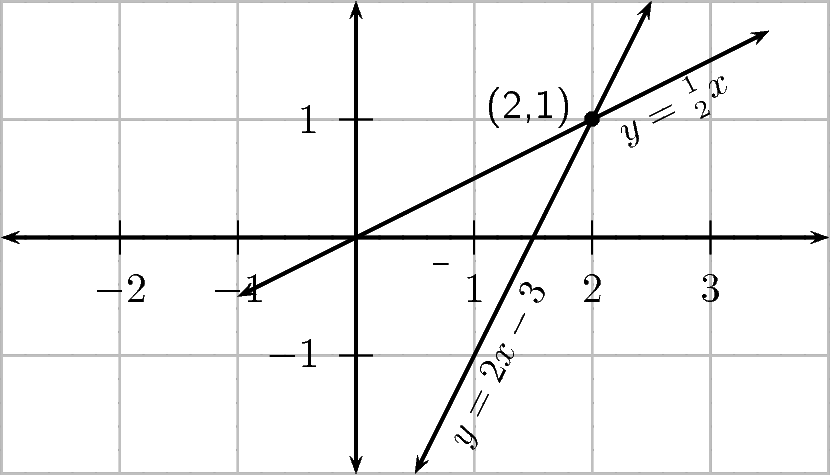
\includegraphics[width=.8\columnwidth]{col11306.imgs/m39257_MG10C10_006.png} % m39257;MG10C10\_006.png;;;6.0;8.5;
\begin{pspicture}(-3,-2)(4,2)
\psgrid[gridcolor=lightgray,gridlabels=0,gridwidth=0.5pt]
\psaxes[dx=1,Dx=1,arrows=<->](0,0)(-3,-2)(4,2)
\pstextpath[c](-1.1,-0.3){\psplot[xunit=1,plotstyle=curve,arrows=<->]{0.5}{2.5}{x 2 mul 3 sub}}{\small{$y=2x-3$}}
\pstextpath[c](1.5,-0.3){\psplot[xunit=1,plotstyle=curve,arrows=<->]{-1}{3.5}{0.5 x mul}}{\small{$y=\frac{1}{2}x$}}
\uput[l](2,1.1){(2,1)}
\psdot(2,1)
\end{pspicture}
      \vspace{2pt}
    \vspace{.1in}
    \rule[.1in]{\figurerulewidth}{.005in} \\
    \end{center}
 \end{figure}       
        \label{m39257*id159137}The intersection of the two graphs is $\left(2,1\right)$. So the solution to the system of simultaneous equations in (9.65) is $y=1$ and $x=2$.\par 
        \label{m39257*id159194}This can be shown algebraically as:\par 
        \label{m39257*id159197}\nopagebreak\noindent{}
    \begin{equation}
    \begin{array}{ccc}\hfill x& =& 2y\hfill \\ \hfill \^{a}ˆ´y& =& 2\left(2y\right)-3\hfill \\ \hfill y-4y& =& -3\hfill \\ \hfill -3y& =& -3\hfill \\ \hfill y& =& 1\hfill \\ \hfill \mathrm{Substitute\; into\; the\; first\; equation:}\phantom{\rule{2.em}{0ex}}\mathrm{x}& =& 2\left(1\right)\hfill \\ & =& 2\hfill \end{array}\tag{9.66}
      \end{equation}
\par
            \label{m39257*secfhsst!!!underscore!!!id4743}\vspace{.5cm} 
      \noindent
      \hspace*{-30pt}
\includegraphics[width=0.5in]{col11306.imgs/pspencil2.png}   \raisebox{25mm}{   
      \begin{mdframed}[linewidth=4, leftmargin=40, rightmargin=40]  
      \begin{exercise}
    \noindent\textbf{Exercise 9.14:  Simultaneous Equations }
        \label{m39257*probfhsst!!!underscore!!!id4744}
        \label{m39257*id159395}Solve the following system of simultaneous equations graphically.\par 
        \label{m39257*id159402}\nopagebreak\noindent{}
          
    \begin{equation}
    \begin{array}{ccc}\hfill 4y+3x& =& 100\hfill \\ \hfill 4y-19x& =& 12\hfill \end{array}\tag{9.67}
      \end{equation}
        \vspace{5pt}
        \label{m39257*solfhsst!!!underscore!!!id4788}\noindent\textbf{Solution to Exercise } \label{m39257*listfhsst!!!underscore!!!id4788}\begin{enumerate}[noitemsep, label=\textbf{Step} \textbf{\arabic*}. ] 
            \leftskip=20pt\rightskip=\leftskip\item  
        \label{m39257*id159487}For the first equation:\par 
        \label{m39257*id159491}\nopagebreak\noindent{}
          
    \begin{equation}
    \begin{array}{ccc}\hfill 4y+3x& =& 100\hfill \\ \hfill 4y& =& 100-3x\hfill \\ \hfill y& =& 25-\frac{3}{4}x\hfill \end{array}\tag{9.68}
      \end{equation}
        \label{m39257*id159580}and for the second equation:\par 
        \label{m39257*id159586}\nopagebreak\noindent{}
          
    \begin{equation}
    \begin{array}{ccc}\hfill 4y-19x& =& 12\hfill \\ \hfill 4y& =& 19x+12\hfill \\ \hfill y& =& \frac{19}{4}x+3\hfill \end{array}\tag{9.69}
      \end{equation}
        \label{m39257*id159676}
    \setcounter{subfigure}{0}
	\begin{figure}[H] % horizontal\label{m39257*id159679}
    \begin{center}
    \label{m39257*id159679!!!underscore!!!media}\label{m39257*id159679!!!underscore!!!printimage}
%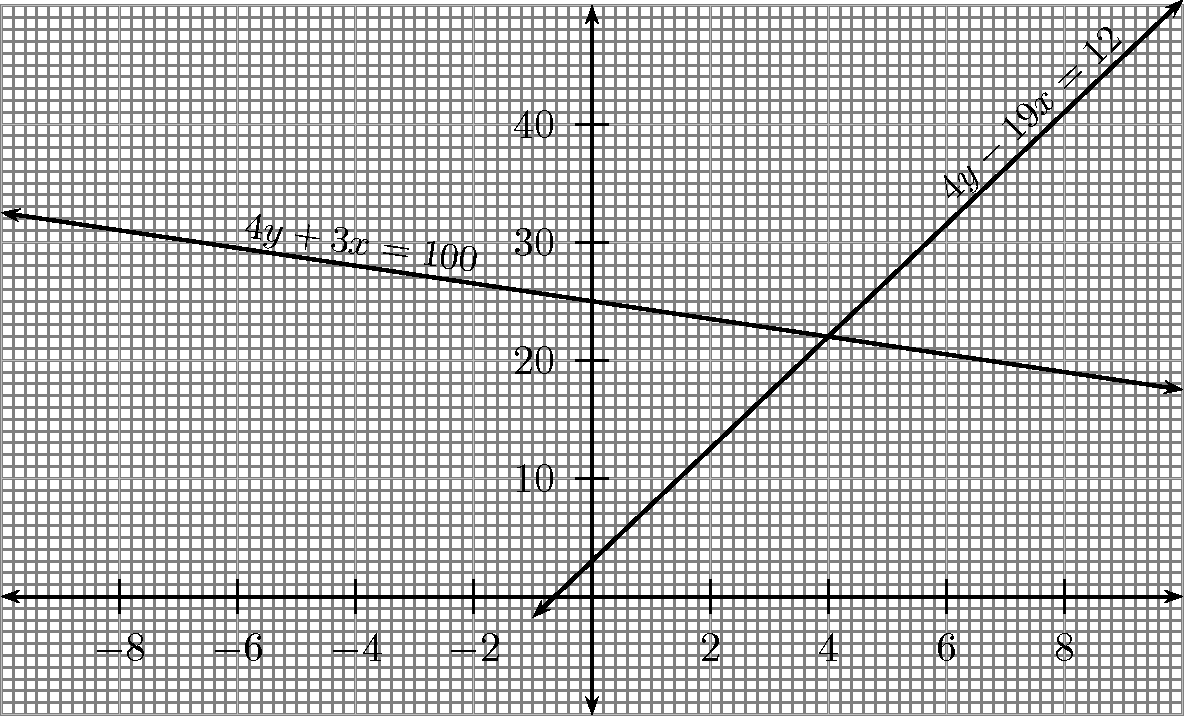
\includegraphics{col11306.imgs/m39257_MG10C10_007.png} % ;MG10C10\_007.png;;;6.0;8.5;
\begin{center}
\begin{pspicture}(-5,-1)(5,5)
\psgrid[subgriddiv=10,gridcolor=lightgray,gridlabels=0,gridwidth=0.1pt]
\psaxes[dx=1,dy=1,Dy=10,Dx=2,arrows=<->](0,0)(-5,-1)(5,5)
\pstextpath[c](-2,0.1){\psplot[xunit=0.5,yunit=0.1,plotstyle=curve,arrows=<->]{-10}{10}{0.75 x mul neg 25 add}}{\small{$4y+3x=100$}}
\pstextpath[c](2.2,0.1){\psplot[xunit=0.5,yunit=0.1,plotstyle=curve,arrows=<->]{-1}{10}{4.75 x mul 3 add}}{\small{$4y-19x=12$}}
\end{pspicture}
\end{center}

      \vspace{2pt}
    \vspace{.1in}
    \end{center}
 \end{figure}       
        \par 
        \item  
        \label{m39257*id159690}The graphs intersect at $\left(4,22\right)$.\par 
        \item  
        \label{m39257*id159717}\nopagebreak\noindent{}
          
    \begin{equation}
    \begin{array}{ccc}\hfill x& =& 4\hfill \\ \hfill y& =& 22\hfill \end{array}\tag{9.70}
      \end{equation}
        \end{enumerate}
    \end{exercise}
    \end{mdframed}
    }
    \noindent
\par
    \noindent
\label{m39257*secfhsst!!!underscore!!!id5809}
            \subsubsection{ Exercise: Simultaneous Equations }
            \nopagebreak
        \label{m39257*id161286}\begin{enumerate}[noitemsep, label=\textbf{\arabic*}. ] 
            \label{m39257*uid98}\item Solve graphically and confirm your answer algebraically:
$3a-2b7=0$ , $a-4b+1=0$\hspace{1ex}        
\label{m39257*uid99}\item Solve algebraically: $15c+11d-132=0$, $2c+3d-59=0$\hspace{1ex}        
\label{m39257*uid100}\item Solve algebraically: $-18e-18+3f=0$, $e-4f+47=0$\hspace{1ex}        
\label{m39257*uid101}\item Solve graphically: $x+2y=7$, $x+y=0$\hspace{1ex}        
\end{enumerate}
\label{m39257**end}
\par \raisebox{-5 pt}{
\includegraphics[width=0.5cm]{col11306.imgs/summary_www.png}} Find the answers with the shortcodes:
 \par \begin{tabular}[h]{cccccc}
 (1.) lxq  &  (2.) lxl  &  (3.) lxi  &  (4.) lx3  & \end{tabular}
        \section{ Word Problems}
    \nopagebreak
            \label{m39262} $ \hspace{-5pt}\begin{array}{cccccccccccc}   
\includegraphics[width=0.75cm]{col11306.imgs/summary_fullmarks.png} &   \end{array} $ \hspace{2 pt}\raisebox{-5 pt}{} {(section shortcode: MG10079 )} \par 
%   
% \label{m39262*cid8}
%             \subsection{ Equations and inequalities: Mathematical models}
%             \nopagebreak
% \label{m39262*uid102}
%             \subsubsection{ Introduction}
%             \nopagebreak
%             
        \label{m39262*id161557}Tom and Jane are friends. Tom picked up Jane's Physics test paper, but will not tell Jane what her marks are. He knows that Jane hates maths so he decided to tease her. Tom says: 'I have 2 marks more than you do and the sum of both our marks is equal to 14. How much did we get?'\par 
        \label{m39262*id161565}Let's help Jane find out what her marks are. We have two unknowns, Tom's mark (which we shall call $t$) and Jane's mark (which we shall call $j$). Tom has 2 more marks than Jane. Therefore,\par 
        \label{m39262*id161587}\nopagebreak\noindent{}
          
    \begin{equation}
    t=j+2\tag{9.84}
      \end{equation}
        \label{m39262*id161608}Also, both marks add up to 14. Therefore,\par 
        \label{m39262*id161614}\nopagebreak\noindent{}
          
    \begin{equation}
    t+j=14\tag{9.85}
      \end{equation}
        \label{m39262*id161635}The two equations make up a set of linear (because the highest power is one) simultaneous equations, which we know how to solve! Substitute for $t$ in the second equation to get:\par 
        \label{m39262*id161648}\nopagebreak\noindent{}
          
    \begin{equation}
    \begin{array}{ccc}\hfill t+j& =& 14\hfill \\ \hfill j+2+j& =& 14\hfill \\ \hfill 2j+2& =& 14\hfill \\ \hfill 2\left(j+1\right)& =& 14\hfill \\ \hfill j+1& =& 7\hfill \\ \hfill j& =& 7-1\hfill \\ & =& 6\hfill \end{array}\tag{9.86}
      \end{equation}
        \label{m39262*id161806}Then,\par 
        \label{m39262*id161812}\nopagebreak\noindent{}
          
    \begin{equation}
    \begin{array}{ccc}\hfill t& =& j+2\hfill \\ & =& 6+2\hfill \\ & =& 8\hfill \end{array}\tag{9.87}
      \end{equation}
        \label{m39262*id161871}So, we see that Tom scored 8 on his test and Jane scored 6.\par 
        \label{m39262*id161878}This problem is an example of a simple \textsl{mathematical model}. We took a problem and we were able to write a set of equations that represented the problem mathematically. The solution of the equations then gave the solution to the problem.\par 
      \label{m39262*uid103}
            \subsubsubsection{ Problem Solving Strategy}
            \nopagebreak
        \label{m39262*id161898}The purpose of this section is to teach you the skills that you need to be able to take a problem and formulate it mathematically in order to solve it. The general steps to follow are:\par 
        \label{m39262*id161903}\begin{enumerate}[noitemsep, label=\textbf{\arabic*}. ] 
            \label{m39262*uid104}\item Read ALL of the question !
\label{m39262*uid105}\item Find out what is requested.
\label{m39262*uid106}\item Use a variable(s) to denote the unknown quantity/quantities that has/have been requested e.g., $x$.
\label{m39262*uid107}\item Rewrite the information given in terms of the variable(s). That is, translate the words into algebraic expressions. 
\label{m39262*uid108}\item Set up an equation or set of equations (i.e. a mathematical sentence or model) to solve the required variable.
\label{m39262*uid109}\item Solve the equation algebraically to find the result.
\end{enumerate}
      \label{m39262*uid110}
            \subsubsection{ Application of Word Problems}
            \nopagebreak
            \par
            \label{m39262*secfhsst!!!underscore!!!id6176}\vspace{.5cm} 
      \noindent
      \hspace*{-30pt}
\includegraphics[width=0.5in]{col11306.imgs/pspencil2.png}   \raisebox{25mm}{   
      \begin{mdframed}[linewidth=4, leftmargin=40, rightmargin=40]  
      \begin{exercise}
    \noindent\textbf{Exercise 9.18:  Mathematical Modelling: Two variables }
        \label{m39262*probfhsst!!!underscore!!!id6177}
        \label{m39262*id162387}Three rulers and two pens have a total cost of R 21,00. One ruler and one pen have a total cost of R 8,00. How much does a ruler costs on its own and how much does a pen cost on its own? \par 
        \vspace{5pt}
        \label{m39262*solfhsst!!!underscore!!!id6180}\noindent\textbf{Solution to Exercise } \label{m39262*listfhsst!!!underscore!!!id6180}\begin{enumerate}[noitemsep, label=\textbf{Step} \textbf{\arabic*}. ] 
            \leftskip=20pt\rightskip=\leftskip\item  
        \label{m39262*id162412}Let the cost of one ruler be $x$ rand and the cost of one pen be $y$ rand.\par 
        \item  
        \label{m39262*uid111}\nopagebreak\noindent{}
          
    \begin{equation}
    \begin{array}{ccc}\hfill 3x+2y& =& 21\hfill \\ \hfill x+y& =& 8\hfill \end{array}\tag{9.88}
      \end{equation}
        \item  
        \label{m39262*id162503}First solve the second equation for $y$:\par 
        \label{m39262*id162516}\nopagebreak\noindent{}
          
    \begin{equation}
    y=8-x\tag{9.89}
      \end{equation}
        \label{m39262*id162536}and substitute the result into the first equation:\par 
        \label{m39262*id162542}\nopagebreak\noindent{}
          
    \begin{equation}
    \begin{array}{ccc}\hfill 3x+2\left(8-x\right)& =& 21\hfill \\ \hfill 3x+16-2x& =& 21\hfill \\ \hfill x& =& 5\hfill \end{array}\tag{9.90}
      \end{equation}
        \label{m39262*id162631}therefore\par 
        \label{m39262*id162637}\nopagebreak\noindent{}
          
    \begin{equation}
    \begin{array}{ccc}\hfill y& =& 8-5\hfill \\ \hfill y& =& 3\hfill \end{array}\tag{9.91}
      \end{equation}
        \item  
        \label{m39262*id162689}\ensuremath{\hat{A}}~\ensuremath{\hat{A}}~\ensuremath{\hat{A}}~\ensuremath{\hat{A}}~\ensuremath{\hat{A}}~\ensuremath{\hat{A}}~\ensuremath{\hat{A}}~\ensuremath{\hat{A}}~\ensuremath{\hat{A}}~\ensuremath{\hat{A}}~\ensuremath{\hat{A}}~\ensuremath{\hat{A}}~One ruler costs R 5,00 and one pen costs R 3,00.
 \par 
        \end{enumerate}
    \end{exercise}
    \end{mdframed}
    }
 \label{m39257*secfhsst!!!underscore!!!id5599}\vspace{.5cm} 
      \noindent
      \hspace*{-30pt}
\includegraphics[width=0.5in]{col11306.imgs/pspencil2.png}   \raisebox{25mm}{   
      \begin{mdframed}[linewidth=4, leftmargin=40, rightmargin=40]  
      \begin{exercise}
    \noindent\textbf{Exercise 9.16:  Bicycles and Tricycles }
        \label{m39257*probfhsst!!!underscore!!!id5600}
        \label{m39257*id160890}A shop sells bicycles and tricycles. In total there are 7 cycles (cycles includes both bicycles and tricycles) and 19 wheels. Determine how many of each there are, if a bicycle has two wheels and a tricycle has three wheels. \par 
        \vspace{5pt}
        \label{m39257*solfhsst!!!underscore!!!id5603}\noindent\textbf{Solution to Exercise } \label{m39257*listfhsst!!!underscore!!!id5603}\begin{enumerate}[noitemsep, label=\textbf{Step} \textbf{\arabic*}. ] 
            \leftskip=20pt\rightskip=\leftskip\item  
        \label{m39257*id160915}The number of bicycles and the number of tricycles are required.\par 
        \item  
        \label{m39257*id160923}If $b$ is the number of bicycles and $t$ is the number of tricycles, then:\par 
        \label{m39257*id160945}\nopagebreak\noindent{}
          
    \begin{equation}
    \begin{array}{ccc}\hfill b+t& =& 7\hfill \\ \hfill 2b+3t& =& 19\hfill \end{array}\tag{9.80}
      \end{equation}
        \item  
        \label{m39257*id161006}\nopagebreak\noindent{}
    \begin{equation}
    \begin{array}{ccc}\hfill b& =& 7-t\hfill \\ \hfill \mathrm{Into\; second\; equation:}2\left(7-\mathrm{t}\right)+3\mathrm{t}& =& 19\hfill \\ \hfill 14-2t+3t& =& 19\hfill \\ \hfill t& =& 5\hfill \\ \hfill \mathrm{Into\; first\; equation:}:\mathrm{b}& =& 7-5\hfill \\ & =& 2\hfill \end{array}\tag{9.81}
      \end{equation}
        \item  
        \label{m39257*id161187}\nopagebreak\noindent{}
          
    \begin{equation}
    \begin{array}{ccc}\hfill 2+5& =& 7\hfill \\ \hfill 2\left(2\right)+3\left(5\right)=4+15& =& 19\hfill \end{array}\tag{9.82}
      \end{equation}
        \end{enumerate}
 \par        
    \end{exercise}
    \end{mdframed}
    }
    \noindent
\label{m39262*secfhsst!!!underscore!!!id6031}\vspace{.5cm} 
      \noindent
      \hspace*{-30pt}
\includegraphics[width=0.5in]{col11306.imgs/pspencil2.png}   \raisebox{25mm}{   
      \begin{mdframed}[linewidth=4, leftmargin=40, rightmargin=40]  
      \begin{exercise}
    \noindent\textbf{Exercise 9.19: Mathematical Modelling: One variable }\label{m39262*probfhsst!!!underscore!!!id6032}
        \label{m39262*id162036}A fruit shake costs R2,00 more than a chocolate milkshake. If three fruit shakes and 5 chocolate milkshakes cost R78,00, determine the individual prices. \par 
        \vspace{5pt}
        \label{m39262*solfhsst!!!underscore!!!id6035}\noindent\textbf{Solution to Exercise } \label{m39262*listfhsst!!!underscore!!!id6035}\begin{enumerate}[noitemsep, label=\textbf{Step} \textbf{\arabic*}. ] 
            \leftskip=20pt\rightskip=\leftskip\item  
        \label{m39262*eip-121}Let the price of a chocolate milkshake be $x$ and the price of a fruitshake be $y$.\par 
    % \textbf{m39262*id162061}\par
    % how many colspecs?  4
          % name: cnx:colspec
            % colnum: 1
            % colwidth: 10*
            % latex-name: columna
            % colname: 
            % align/tgroup-align/default: //left
            % -------------------------
            % name: cnx:colspec
            % colnum: 2
            % colwidth: 10*
            % latex-name: columnb
            % colname: 
            % align/tgroup-align/default: //left
            % -------------------------
            % name: cnx:colspec
            % colnum: 3
            % colwidth: 10*
            % latex-name: columnc
            % colname: 
            % align/tgroup-align/default: //left
            % -------------------------
            % name: cnx:colspec
            % colnum: 4
            % colwidth: 10*
            % latex-name: columnd
            % colname: 
            % align/tgroup-align/default: //left
            % -------------------------
    \setlength\mytablespace{8\tabcolsep}
    \addtolength\mytablespace{5\arrayrulewidth}
    \setlength\mytablewidth{\linewidth}
    \setlength\mytableroom{\mytablewidth}
    \addtolength\mytableroom{-\mytablespace}
    \setlength\myfixedwidth{0pt}
    \setlength\mystarwidth{\mytableroom}
        \addtolength\mystarwidth{-\myfixedwidth}
        \divide\mystarwidth 40
      % ----- Begin capturing width of table in LR mode woof
      \settowidth{\mytableboxwidth}{\begin{tabular}[t]{|l|l|l|l|}\hline
    % count in rowspan-info-nodeset: 4
    % align/colidx: left,1
    % rowcount: '0' | start: 'false' | colidx: '1'
        % Formatting a regular cell and recurring on the next sibling
         &
      % align/colidx: left,2
    % rowcount: '0' | start: 'false' | colidx: '2'
        % Formatting a regular cell and recurring on the next sibling
        Price &
      % align/colidx: left,3
    % rowcount: '0' | start: 'false' | colidx: '3'
        % Formatting a regular cell and recurring on the next sibling
        number &
      % align/colidx: left,4
    % rowcount: '0' | start: 'false' | colidx: '4'
        % Formatting a regular cell and recurring on the next sibling
        Total% make-rowspan-placeholders
    % rowspan info: col1 '0' | 'false' | '' || col2 '0' | 'false' | '' || col3 '0' | 'false' | '' || col4 '0' | 'false' | ''
     \tabularnewline\cline{1-1}\cline{2-2}\cline{3-3}\cline{4-4}
      %--------------------------------------------------------------------
    % align/colidx: left,1
    % rowcount: '0' | start: 'false' | colidx: '1'
        % Formatting a regular cell and recurring on the next sibling
        Fruit &
      % align/colidx: left,2
    % rowcount: '0' | start: 'false' | colidx: '2'
        % Formatting a regular cell and recurring on the next sibling
                  $y$
                 &
      % align/colidx: left,3
    % rowcount: '0' | start: 'false' | colidx: '3'
        % Formatting a regular cell and recurring on the next sibling
        3 &
      % align/colidx: left,4
    % rowcount: '0' | start: 'false' | colidx: '4'
        % Formatting a regular cell and recurring on the next sibling
                  $3y$
                % make-rowspan-placeholders
    % rowspan info: col1 '0' | 'false' | '' || col2 '0' | 'false' | '' || col3 '0' | 'false' | '' || col4 '0' | 'false' | ''
     \tabularnewline\cline{1-1}\cline{2-2}\cline{3-3}\cline{4-4}
      %--------------------------------------------------------------------
    % align/colidx: left,1
    % rowcount: '0' | start: 'false' | colidx: '1'
        % Formatting a regular cell and recurring on the next sibling
        Chocolate &
      % align/colidx: left,2
    % rowcount: '0' | start: 'false' | colidx: '2'
        % Formatting a regular cell and recurring on the next sibling
                  $x$
                 &
      % align/colidx: left,3
    % rowcount: '0' | start: 'false' | colidx: '3'
        % Formatting a regular cell and recurring on the next sibling
        5 &
      % align/colidx: left,4
    % rowcount: '0' | start: 'false' | colidx: '4'
        % Formatting a regular cell and recurring on the next sibling
                  $5x$
                % make-rowspan-placeholders
    % rowspan info: col1 '0' | 'false' | '' || col2 '0' | 'false' | '' || col3 '0' | 'false' | '' || col4 '0' | 'false' | ''
     \tabularnewline\cline{1-1}\cline{2-2}\cline{3-3}\cline{4-4}
      %--------------------------------------------------------------------
    \end{tabular}} % end mytableboxwidth set      
      % ----- End capturing width of table in LR mode
        % ----- LR or paragraph mode: must test
        % ----- Begin capturing height of table
        \settoheight{\mytableboxheight}{\begin{tabular}[t]{|l|l|l|l|}\hline
    % count in rowspan-info-nodeset: 4
    % align/colidx: left,1
    % rowcount: '0' | start: 'false' | colidx: '1'
        % Formatting a regular cell and recurring on the next sibling
         &
      % align/colidx: left,2
    % rowcount: '0' | start: 'false' | colidx: '2'
        % Formatting a regular cell and recurring on the next sibling
        Price &
      % align/colidx: left,3
    % rowcount: '0' | start: 'false' | colidx: '3'
        % Formatting a regular cell and recurring on the next sibling
        number &
      % align/colidx: left,4
    % rowcount: '0' | start: 'false' | colidx: '4'
        % Formatting a regular cell and recurring on the next sibling
        Total% make-rowspan-placeholders
    % rowspan info: col1 '0' | 'false' | '' || col2 '0' | 'false' | '' || col3 '0' | 'false' | '' || col4 '0' | 'false' | ''
     \tabularnewline\cline{1-1}\cline{2-2}\cline{3-3}\cline{4-4}
      %--------------------------------------------------------------------
    % align/colidx: left,1
    % rowcount: '0' | start: 'false' | colidx: '1'
        % Formatting a regular cell and recurring on the next sibling
        Fruit &
      % align/colidx: left,2
    % rowcount: '0' | start: 'false' | colidx: '2'
        % Formatting a regular cell and recurring on the next sibling
                  $y$
                 &
      % align/colidx: left,3
    % rowcount: '0' | start: 'false' | colidx: '3'
        % Formatting a regular cell and recurring on the next sibling
        3 &
      % align/colidx: left,4
    % rowcount: '0' | start: 'false' | colidx: '4'
        % Formatting a regular cell and recurring on the next sibling
                  $3y$
                % make-rowspan-placeholders
    % rowspan info: col1 '0' | 'false' | '' || col2 '0' | 'false' | '' || col3 '0' | 'false' | '' || col4 '0' | 'false' | ''
     \tabularnewline\cline{1-1}\cline{2-2}\cline{3-3}\cline{4-4}
      %--------------------------------------------------------------------
    % align/colidx: left,1
    % rowcount: '0' | start: 'false' | colidx: '1'
        % Formatting a regular cell and recurring on the next sibling
        Chocolate &
      % align/colidx: left,2
    % rowcount: '0' | start: 'false' | colidx: '2'
        % Formatting a regular cell and recurring on the next sibling
                  $x$
                 &
      % align/colidx: left,3
    % rowcount: '0' | start: 'false' | colidx: '3'
        % Formatting a regular cell and recurring on the next sibling
        5 &
      % align/colidx: left,4
    % rowcount: '0' | start: 'false' | colidx: '4'
        % Formatting a regular cell and recurring on the next sibling
                  $5x$
                % make-rowspan-placeholders
    % rowspan info: col1 '0' | 'false' | '' || col2 '0' | 'false' | '' || col3 '0' | 'false' | '' || col4 '0' | 'false' | ''
     \tabularnewline\cline{1-1}\cline{2-2}\cline{3-3}\cline{4-4}
      %--------------------------------------------------------------------
    \end{tabular}} % end mytableboxheight set
        \settodepth{\mytableboxdepth}{\begin{tabular}[t]{|l|l|l|l|}\hline
    % count in rowspan-info-nodeset: 4
    % align/colidx: left,1
    % rowcount: '0' | start: 'false' | colidx: '1'
        % Formatting a regular cell and recurring on the next sibling
         &
      % align/colidx: left,2
    % rowcount: '0' | start: 'false' | colidx: '2'
        % Formatting a regular cell and recurring on the next sibling
        Price &
      % align/colidx: left,3
    % rowcount: '0' | start: 'false' | colidx: '3'
        % Formatting a regular cell and recurring on the next sibling
        number &
      % align/colidx: left,4
    % rowcount: '0' | start: 'false' | colidx: '4'
        % Formatting a regular cell and recurring on the next sibling
        Total% make-rowspan-placeholders
    % rowspan info: col1 '0' | 'false' | '' || col2 '0' | 'false' | '' || col3 '0' | 'false' | '' || col4 '0' | 'false' | ''
     \tabularnewline\cline{1-1}\cline{2-2}\cline{3-3}\cline{4-4}
      %--------------------------------------------------------------------
    % align/colidx: left,1
    % rowcount: '0' | start: 'false' | colidx: '1'
        % Formatting a regular cell and recurring on the next sibling
        Fruit &
      % align/colidx: left,2
    % rowcount: '0' | start: 'false' | colidx: '2'
        % Formatting a regular cell and recurring on the next sibling
                  $y$
                 &
      % align/colidx: left,3
    % rowcount: '0' | start: 'false' | colidx: '3'
        % Formatting a regular cell and recurring on the next sibling
        3 &
      % align/colidx: left,4
    % rowcount: '0' | start: 'false' | colidx: '4'
        % Formatting a regular cell and recurring on the next sibling
                  $3y$
                % make-rowspan-placeholders
    % rowspan info: col1 '0' | 'false' | '' || col2 '0' | 'false' | '' || col3 '0' | 'false' | '' || col4 '0' | 'false' | ''
     \tabularnewline\cline{1-1}\cline{2-2}\cline{3-3}\cline{4-4}
      %--------------------------------------------------------------------
    % align/colidx: left,1
    % rowcount: '0' | start: 'false' | colidx: '1'
        % Formatting a regular cell and recurring on the next sibling
        Chocolate &
      % align/colidx: left,2
    % rowcount: '0' | start: 'false' | colidx: '2'
        % Formatting a regular cell and recurring on the next sibling
                  $x$
                 &
      % align/colidx: left,3
    % rowcount: '0' | start: 'false' | colidx: '3'
        % Formatting a regular cell and recurring on the next sibling
        5 &
      % align/colidx: left,4
    % rowcount: '0' | start: 'false' | colidx: '4'
        % Formatting a regular cell and recurring on the next sibling
                  $5x$
                % make-rowspan-placeholders
    % rowspan info: col1 '0' | 'false' | '' || col2 '0' | 'false' | '' || col3 '0' | 'false' | '' || col4 '0' | 'false' | ''
     \tabularnewline\cline{1-1}\cline{2-2}\cline{3-3}\cline{4-4}
      %--------------------------------------------------------------------
    \end{tabular}} % end mytableboxdepth set
        \addtolength{\mytableboxheight}{\mytableboxdepth}
        % ----- End capturing height of table        
        \ifthenelse{\mytableboxwidth<\textwidth}{% the table fits in LR mode
          \addtolength{\mytableboxwidth}{-\mytablespace}
          \typeout{textheight: \the\textheight}
          \typeout{mytableboxheight: \the\mytableboxheight}
          \typeout{textwidth: \the\textwidth}
          \typeout{mytableboxwidth: \the\mytableboxwidth}
          \ifthenelse{\mytableboxheight<\textheight}{%
    % \begin{table}[H]
    % \\ 'id2925970' '1'
        \begin{center}
      \label{m39262*id162061}
    \noindent
    \begin{tabular}[t]{|l|l|l|l|}\hline
    % count in rowspan-info-nodeset: 4
    % align/colidx: left,1
    % rowcount: '0' | start: 'false' | colidx: '1'
        % Formatting a regular cell and recurring on the next sibling
         &
      % align/colidx: left,2
    % rowcount: '0' | start: 'false' | colidx: '2'
        % Formatting a regular cell and recurring on the next sibling
        Price &
      % align/colidx: left,3
    % rowcount: '0' | start: 'false' | colidx: '3'
        % Formatting a regular cell and recurring on the next sibling
        number &
      % align/colidx: left,4
    % rowcount: '0' | start: 'false' | colidx: '4'
        % Formatting a regular cell and recurring on the next sibling
        Total% make-rowspan-placeholders
    % rowspan info: col1 '0' | 'false' | '' || col2 '0' | 'false' | '' || col3 '0' | 'false' | '' || col4 '0' | 'false' | ''
     \tabularnewline\cline{1-1}\cline{2-2}\cline{3-3}\cline{4-4}
      %--------------------------------------------------------------------
    % align/colidx: left,1
    % rowcount: '0' | start: 'false' | colidx: '1'
        % Formatting a regular cell and recurring on the next sibling
        Fruit &
      % align/colidx: left,2
    % rowcount: '0' | start: 'false' | colidx: '2'
        % Formatting a regular cell and recurring on the next sibling
                  $y$
                 &
      % align/colidx: left,3
    % rowcount: '0' | start: 'false' | colidx: '3'
        % Formatting a regular cell and recurring on the next sibling
        3 &
      % align/colidx: left,4
    % rowcount: '0' | start: 'false' | colidx: '4'
        % Formatting a regular cell and recurring on the next sibling
                  $3y$
                % make-rowspan-placeholders
    % rowspan info: col1 '0' | 'false' | '' || col2 '0' | 'false' | '' || col3 '0' | 'false' | '' || col4 '0' | 'false' | ''
     \tabularnewline\cline{1-1}\cline{2-2}\cline{3-3}\cline{4-4}
      %--------------------------------------------------------------------
    % align/colidx: left,1
    % rowcount: '0' | start: 'false' | colidx: '1'
        % Formatting a regular cell and recurring on the next sibling
        Chocolate &
      % align/colidx: left,2
    % rowcount: '0' | start: 'false' | colidx: '2'
        % Formatting a regular cell and recurring on the next sibling
                  $x$
                 &
      % align/colidx: left,3
    % rowcount: '0' | start: 'false' | colidx: '3'
        % Formatting a regular cell and recurring on the next sibling
        5 &
      % align/colidx: left,4
    % rowcount: '0' | start: 'false' | colidx: '4'
        % Formatting a regular cell and recurring on the next sibling
                  $5x$
                % make-rowspan-placeholders
    % rowspan info: col1 '0' | 'false' | '' || col2 '0' | 'false' | '' || col3 '0' | 'false' | '' || col4 '0' | 'false' | ''
     \tabularnewline\cline{1-1}\cline{2-2}\cline{3-3}\cline{4-4}
      %--------------------------------------------------------------------
    \end{tabular}
      \end{center}
    \begin{center}{\small\bfseries Table 9.4}\end{center}
    %\end{table}
          }{ % else
    % \begin{table}[H]
    % \\ 'id2925970' '1'
        \begin{center}
      \label{m39262*id162061}
    \noindent
    \tabletail{%
        \hline
        \multicolumn{4}{|p{\mytableboxwidth}|}{\raggedleft \small \sl continued on next page}\\
        \hline
      }
      \tablelasttail{}
      \begin{xtabular}[t]{|l|l|l|l|}\hline
    % count in rowspan-info-nodeset: 4
    % align/colidx: left,1
    % rowcount: '0' | start: 'false' | colidx: '1'
        % Formatting a regular cell and recurring on the next sibling
         &
      % align/colidx: left,2
    % rowcount: '0' | start: 'false' | colidx: '2'
        % Formatting a regular cell and recurring on the next sibling
        Price &
      % align/colidx: left,3
    % rowcount: '0' | start: 'false' | colidx: '3'
        % Formatting a regular cell and recurring on the next sibling
        number &
      % align/colidx: left,4
    % rowcount: '0' | start: 'false' | colidx: '4'
        % Formatting a regular cell and recurring on the next sibling
        Total% make-rowspan-placeholders
    % rowspan info: col1 '0' | 'false' | '' || col2 '0' | 'false' | '' || col3 '0' | 'false' | '' || col4 '0' | 'false' | ''
     \tabularnewline\cline{1-1}\cline{2-2}\cline{3-3}\cline{4-4}
      %--------------------------------------------------------------------
    % align/colidx: left,1
    % rowcount: '0' | start: 'false' | colidx: '1'
        % Formatting a regular cell and recurring on the next sibling
        Fruit &
      % align/colidx: left,2
    % rowcount: '0' | start: 'false' | colidx: '2'
        % Formatting a regular cell and recurring on the next sibling
                  $y$
                 &
      % align/colidx: left,3
    % rowcount: '0' | start: 'false' | colidx: '3'
        % Formatting a regular cell and recurring on the next sibling
        3 &
      % align/colidx: left,4
    % rowcount: '0' | start: 'false' | colidx: '4'
        % Formatting a regular cell and recurring on the next sibling
                  $3y$
                % make-rowspan-placeholders
    % rowspan info: col1 '0' | 'false' | '' || col2 '0' | 'false' | '' || col3 '0' | 'false' | '' || col4 '0' | 'false' | ''
     \tabularnewline\cline{1-1}\cline{2-2}\cline{3-3}\cline{4-4}
      %--------------------------------------------------------------------
    % align/colidx: left,1
    % rowcount: '0' | start: 'false' | colidx: '1'
        % Formatting a regular cell and recurring on the next sibling
        Chocolate &
      % align/colidx: left,2
    % rowcount: '0' | start: 'false' | colidx: '2'
        % Formatting a regular cell and recurring on the next sibling
                  $x$
                 &
      % align/colidx: left,3
    % rowcount: '0' | start: 'false' | colidx: '3'
        % Formatting a regular cell and recurring on the next sibling
        5 &
      % align/colidx: left,4
    % rowcount: '0' | start: 'false' | colidx: '4'
        % Formatting a regular cell and recurring on the next sibling
                  $5x$
                % make-rowspan-placeholders
    % rowspan info: col1 '0' | 'false' | '' || col2 '0' | 'false' | '' || col3 '0' | 'false' | '' || col4 '0' | 'false' | ''
     \tabularnewline\cline{1-1}\cline{2-2}\cline{3-3}\cline{4-4}
      %--------------------------------------------------------------------
    \end{xtabular}
      \end{center}
    \begin{center}{\small\bfseries Table 9.4}\end{center}
    %\end{table}
          } % 
        }{% else
        % typeset the table in paragraph mode
        % ----- Begin capturing height of table
        \settoheight{\mytableboxheight}{\begin{tabular*}{\mytablewidth}[t]{|p{10\mystarwidth}|p{10\mystarwidth}|p{10\mystarwidth}|p{10\mystarwidth}|}\hline
    % count in rowspan-info-nodeset: 4
    % align/colidx: left,1
    % rowcount: '0' | start: 'false' | colidx: '1'
        % Formatting a regular cell and recurring on the next sibling
         &
      % align/colidx: left,2
    % rowcount: '0' | start: 'false' | colidx: '2'
        % Formatting a regular cell and recurring on the next sibling
        Price &
      % align/colidx: left,3
    % rowcount: '0' | start: 'false' | colidx: '3'
        % Formatting a regular cell and recurring on the next sibling
        number &
      % align/colidx: left,4
    % rowcount: '0' | start: 'false' | colidx: '4'
        % Formatting a regular cell and recurring on the next sibling
        Total% make-rowspan-placeholders
    % rowspan info: col1 '0' | 'false' | '' || col2 '0' | 'false' | '' || col3 '0' | 'false' | '' || col4 '0' | 'false' | ''
     \tabularnewline\cline{1-1}\cline{2-2}\cline{3-3}\cline{4-4}
      %--------------------------------------------------------------------
    % align/colidx: left,1
    % rowcount: '0' | start: 'false' | colidx: '1'
        % Formatting a regular cell and recurring on the next sibling
        Fruit &
      % align/colidx: left,2
    % rowcount: '0' | start: 'false' | colidx: '2'
        % Formatting a regular cell and recurring on the next sibling
                  $y$
                 &
      % align/colidx: left,3
    % rowcount: '0' | start: 'false' | colidx: '3'
        % Formatting a regular cell and recurring on the next sibling
        3 &
      % align/colidx: left,4
    % rowcount: '0' | start: 'false' | colidx: '4'
        % Formatting a regular cell and recurring on the next sibling
                  $3y$
                % make-rowspan-placeholders
    % rowspan info: col1 '0' | 'false' | '' || col2 '0' | 'false' | '' || col3 '0' | 'false' | '' || col4 '0' | 'false' | ''
     \tabularnewline\cline{1-1}\cline{2-2}\cline{3-3}\cline{4-4}
      %--------------------------------------------------------------------
    % align/colidx: left,1
    % rowcount: '0' | start: 'false' | colidx: '1'
        % Formatting a regular cell and recurring on the next sibling
        Chocolate &
      % align/colidx: left,2
    % rowcount: '0' | start: 'false' | colidx: '2'
        % Formatting a regular cell and recurring on the next sibling
                  $x$
                 &
      % align/colidx: left,3
    % rowcount: '0' | start: 'false' | colidx: '3'
        % Formatting a regular cell and recurring on the next sibling
        5 &
      % align/colidx: left,4
    % rowcount: '0' | start: 'false' | colidx: '4'
        % Formatting a regular cell and recurring on the next sibling
                  $5x$
                % make-rowspan-placeholders
    % rowspan info: col1 '0' | 'false' | '' || col2 '0' | 'false' | '' || col3 '0' | 'false' | '' || col4 '0' | 'false' | ''
     \tabularnewline\cline{1-1}\cline{2-2}\cline{3-3}\cline{4-4}
      %--------------------------------------------------------------------
    \end{tabular*}} % end mytableboxheight set
        \settodepth{\mytableboxdepth}{\begin{tabular*}{\mytablewidth}[t]{|p{10\mystarwidth}|p{10\mystarwidth}|p{10\mystarwidth}|p{10\mystarwidth}|}\hline
    % count in rowspan-info-nodeset: 4
    % align/colidx: left,1
    % rowcount: '0' | start: 'false' | colidx: '1'
        % Formatting a regular cell and recurring on the next sibling
         &
      % align/colidx: left,2
    % rowcount: '0' | start: 'false' | colidx: '2'
        % Formatting a regular cell and recurring on the next sibling
        Price &
      % align/colidx: left,3
    % rowcount: '0' | start: 'false' | colidx: '3'
        % Formatting a regular cell and recurring on the next sibling
        number &
      % align/colidx: left,4
    % rowcount: '0' | start: 'false' | colidx: '4'
        % Formatting a regular cell and recurring on the next sibling
        Total% make-rowspan-placeholders
    % rowspan info: col1 '0' | 'false' | '' || col2 '0' | 'false' | '' || col3 '0' | 'false' | '' || col4 '0' | 'false' | ''
     \tabularnewline\cline{1-1}\cline{2-2}\cline{3-3}\cline{4-4}
      %--------------------------------------------------------------------
    % align/colidx: left,1
    % rowcount: '0' | start: 'false' | colidx: '1'
        % Formatting a regular cell and recurring on the next sibling
        Fruit &
      % align/colidx: left,2
    % rowcount: '0' | start: 'false' | colidx: '2'
        % Formatting a regular cell and recurring on the next sibling
                  $y$
                 &
      % align/colidx: left,3
    % rowcount: '0' | start: 'false' | colidx: '3'
        % Formatting a regular cell and recurring on the next sibling
        3 &
      % align/colidx: left,4
    % rowcount: '0' | start: 'false' | colidx: '4'
        % Formatting a regular cell and recurring on the next sibling
                  $3y$
                % make-rowspan-placeholders
    % rowspan info: col1 '0' | 'false' | '' || col2 '0' | 'false' | '' || col3 '0' | 'false' | '' || col4 '0' | 'false' | ''
     \tabularnewline\cline{1-1}\cline{2-2}\cline{3-3}\cline{4-4}
      %--------------------------------------------------------------------
    % align/colidx: left,1
    % rowcount: '0' | start: 'false' | colidx: '1'
        % Formatting a regular cell and recurring on the next sibling
        Chocolate &
      % align/colidx: left,2
    % rowcount: '0' | start: 'false' | colidx: '2'
        % Formatting a regular cell and recurring on the next sibling
                  $x$
                 &
      % align/colidx: left,3
    % rowcount: '0' | start: 'false' | colidx: '3'
        % Formatting a regular cell and recurring on the next sibling
        5 &
      % align/colidx: left,4
    % rowcount: '0' | start: 'false' | colidx: '4'
        % Formatting a regular cell and recurring on the next sibling
                  $5x$
                % make-rowspan-placeholders
    % rowspan info: col1 '0' | 'false' | '' || col2 '0' | 'false' | '' || col3 '0' | 'false' | '' || col4 '0' | 'false' | ''
     \tabularnewline\cline{1-1}\cline{2-2}\cline{3-3}\cline{4-4}
      %--------------------------------------------------------------------
    \end{tabular*}} % end mytableboxdepth set
        \addtolength{\mytableboxheight}{\mytableboxdepth}
        % ----- End capturing height of table
        \typeout{textheight: \the\textheight}
        \typeout{mytableboxheight: \the\mytableboxheight}
        \typeout{table too wide, outputting in para mode}
    % \begin{table}[H]
    % \\ 'id2925970' '1'
        \begin{center}
      \label{m39262*id162061}
    \noindent
    \tabletail{%
        \hline
        \multicolumn{4}{|p{\mytableroom}|}{\raggedleft \small \sl continued on next page}\\
        \hline
      }
      \tablelasttail{}
      \begin{xtabular*}{\mytablewidth}[t]{|p{10\mystarwidth}|p{10\mystarwidth}|p{10\mystarwidth}|p{10\mystarwidth}|}\hline
    % count in rowspan-info-nodeset: 4
    % align/colidx: left,1
    % rowcount: '0' | start: 'false' | colidx: '1'
        % Formatting a regular cell and recurring on the next sibling
         &
      % align/colidx: left,2
    % rowcount: '0' | start: 'false' | colidx: '2'
        % Formatting a regular cell and recurring on the next sibling
        Price &
      % align/colidx: left,3
    % rowcount: '0' | start: 'false' | colidx: '3'
        % Formatting a regular cell and recurring on the next sibling
        number &
      % align/colidx: left,4
    % rowcount: '0' | start: 'false' | colidx: '4'
        % Formatting a regular cell and recurring on the next sibling
        Total% make-rowspan-placeholders
    % rowspan info: col1 '0' | 'false' | '' || col2 '0' | 'false' | '' || col3 '0' | 'false' | '' || col4 '0' | 'false' | ''
     \tabularnewline\cline{1-1}\cline{2-2}\cline{3-3}\cline{4-4}
      %--------------------------------------------------------------------
    % align/colidx: left,1
    % rowcount: '0' | start: 'false' | colidx: '1'
        % Formatting a regular cell and recurring on the next sibling
        Fruit &
      % align/colidx: left,2
    % rowcount: '0' | start: 'false' | colidx: '2'
        % Formatting a regular cell and recurring on the next sibling
                  $y$
                 &
      % align/colidx: left,3
    % rowcount: '0' | start: 'false' | colidx: '3'
        % Formatting a regular cell and recurring on the next sibling
        3 &
      % align/colidx: left,4
    % rowcount: '0' | start: 'false' | colidx: '4'
        % Formatting a regular cell and recurring on the next sibling
                  $3y$
                % make-rowspan-placeholders
    % rowspan info: col1 '0' | 'false' | '' || col2 '0' | 'false' | '' || col3 '0' | 'false' | '' || col4 '0' | 'false' | ''
     \tabularnewline\cline{1-1}\cline{2-2}\cline{3-3}\cline{4-4}
      %--------------------------------------------------------------------
    % align/colidx: left,1
    % rowcount: '0' | start: 'false' | colidx: '1'
        % Formatting a regular cell and recurring on the next sibling
        Chocolate &
      % align/colidx: left,2
    % rowcount: '0' | start: 'false' | colidx: '2'
        % Formatting a regular cell and recurring on the next sibling
                  $x$
                 &
      % align/colidx: left,3
    % rowcount: '0' | start: 'false' | colidx: '3'
        % Formatting a regular cell and recurring on the next sibling
        5 &
      % align/colidx: left,4
    % rowcount: '0' | start: 'false' | colidx: '4'
        % Formatting a regular cell and recurring on the next sibling
                  $5x$
                % make-rowspan-placeholders
    % rowspan info: col1 '0' | 'false' | '' || col2 '0' | 'false' | '' || col3 '0' | 'false' | '' || col4 '0' | 'false' | ''
     \tabularnewline\cline{1-1}\cline{2-2}\cline{3-3}\cline{4-4}
      %--------------------------------------------------------------------
    \end{xtabular*}
      \end{center}
    \begin{center}{\small\bfseries Table 9.4}\end{center}
    %\end{table}
        }% ending lr/para test clause
    \par
        \item  
        \label{m39262*id162231}\nopagebreak\noindent{}
          
    \begin{equation}
    \begin{array}{ccc}\hfill 3y+5x& =& 78\hfill \end{array}\tag{9.92}
      \end{equation}
        \label{m39262*eip-840}$y=x+2$\par 
        \item  
        \label{m39262*id162280}\nopagebreak\noindent{}
    \begin{equation}
    \begin{array}{ccc}\hfill 3\left(x+2\right)+5x& =& 78\hfill \\ \hfill 3x+6+5x& =& 78\hfill \\ \hfill 8x& =& 72\hfill \\ \hfill x& =& 9\hfill \\ \hfill y& =& x+2\hfill \\ \hfill & =& 9+2\hfill \\ \hfill & =& 11\hfill \end{array}\tag{9.93}
      \end{equation}
        \item  
        \label{m39262*id162358}One chocolate milkshake costs R 9,00 and one Fruitshake costs R 11,00
 \par 
        \end{enumerate}
    \end{exercise}
    \end{mdframed}
    }
    \noindent
\label{m39262*secfhsst!!!underscore!!!id6331}
            \subsubsection{Exercise:  Word Problems }
            \nopagebreak
        \label{m39262*id162712}\begin{enumerate}[noitemsep, label=\textbf{\arabic*}. ] 
            \label{m39262*uid112}\item Stephen has 1\ensuremath{\hat{A}}~l of a mixture containing 69\% of salt. How much water must Stephen add to make the mixture 50\% salt? Write your answer as a fraction of a litre.
\hspace{1ex}        
\label{m39262*uid113}\item The diagonal of a rectangle is 25\ensuremath{\hat{A}}~cm more than its width. The length of the rectangle is 17\ensuremath{\hat{A}}~cm more than its width. What are the dimensions of the rectangle?
\hspace{1ex}        
\label{m39262*uid114}\item The sum of 27 and 12 is 73 more than an unknown number. Find the unknown number.
\hspace{1ex}        
\label{m39262*uid115}\item The two smaller angles in a right-angled triangle are in the ratio of 1:2. What are the sizes of the two angles?
\hspace{1ex}        
\label{m39262*uid116}\item George owns a bakery that specialises in wedding cakes. For each wedding cake, it costs George R150 for ingredients, R50 for overhead, and R5 for advertising. George's wedding cakes cost R400 each. As a percentage of George's costs, how much profit does he make for each cake sold?
\hspace{1ex}        
\label{m39262*uid117}\item If 4 times a number is increased by 7, the result is 15 less than the square of the number. Find the numbers that satisfy this statement, by formulating an equation and then solving it.
\hspace{1ex}        
\label{m39262*uid118}\item The length of a rectangle is 2\ensuremath{\hat{A}}~cm more than the width of the rectangle. The perimeter of the rectangle is 20\ensuremath{\hat{A}}~cm. Find the length and the width of the rectangle.
\hspace{1ex}        
\end{enumerate}
\label{m39262**end}
\par \raisebox{-5 pt}{
\includegraphics[width=0.5cm]{col11306.imgs/summary_www.png}} Find the answers with the shortcodes:
 \par \begin{tabular}[h]{cccccc}
 (1.) lcy  &  (2.) lcV  &  (3.) lcp  &  (4.) lcw  &  (5.) lcd  &  (6.) lcf  &  (7.) lcv  & \end{tabular}
         \section{ Literal equations}
    \nopagebreak
            \label{m39258} $ \hspace{-5pt}\begin{array}{cccccccccccc}   
\includegraphics[width=0.75cm]{col11306.imgs/summary_fullmarks.png} &   \end{array} $ \hspace{2 pt}\raisebox{-5 pt}{} {(section shortcode: MG10078 )} \par 
%   \label{m39258*eip-798}
%             \ssection{ Equations and inequalities: Literal equations}
%             \nopagebreak
%             
\label{m39258*eip-224}A literal equation is one that has several letters or variables. Examples include the area of a circle ($A=\mathrm{Ï€}{r}^{2}$) and the formula for speed ($s=\frac{d}{t}$). In this section you will learn how to solve literal equations in terms of one variable. To do this, you will use the principles you have learnt about solving equations and apply them to rearranging literal equations. Solving literal equations is also known as changing the subject of the formula.
\par 
\label{m39258*id9732423}
You should bear the following in mind when solving literal equations: \label{m39258*id987324}\begin{itemize}[noitemsep]
            \item We isolate the unknown by asking what is joined to it, how this is joined and we do the opposite operation (to both sides as a whole).
\item If the unknown variable is in two or more terms, then we take it out as a common factor. 
\item  If we have to take the square root of both sides, remember that there will be a positive and a negative answer.
\item  If the unknown variable is in the denominator, then we find the lowest common denominator (LCD), multiply both sides by LCD and then continue to solve the problem.
\end{itemize}
\par 
\par
            \label{m39258*eip-979}\vspace{.5cm} 
      \noindent
      \hspace*{-30pt}
\includegraphics[width=0.5in]{col11306.imgs/pspencil2.png}   \raisebox{25mm}{   
      \begin{mdframed}[linewidth=4, leftmargin=40, rightmargin=40]  
      \begin{exercise}
    \noindent\textbf{Exercise 9.17: Solving literal equations - 1}\label{m39258*probfhsst!!!underscore!!!id64377}
        \label{m39258*id162453587}The area of a triangle is $A=\frac{1}{2}bÃ---h$. What is the height of the triangle in terms of the base and area?\par 
        \vspace{5pt}
        \label{m39258*solfhsst!!!underscore!!!id66480}\noindent\textbf{Solution to Exercise } \label{m39258*listfhsst!!!underscore!!!id63453480}\begin{enumerate}[noitemsep, label=\textbf{Step} \textbf{\arabic*}. ] 
            \leftskip=20pt\rightskip=\leftskip\item  We rearrange the equation so that the height is on one side of the equals sign and the rest of the variables are on the other side of the equation.
        \label{m39258*uid5665411}\nopagebreak\noindent{}
    \begin{equation}
    \begin{array}{cccc}\hfill A& =& \frac{1}{2}bÃ---h\hfill & \\ \hfill 2A& =& bÃ---h\hfill & \left(\mathrm{multiply\; both\; sides\; by\; 2}\right)\hfill \\ \hfill \frac{2A}{b}& =& h\hfill & \left(\mathrm{divide\; both\; sides\; by\; b}\right)\hfill \end{array}\tag{9.83}
      \end{equation}
        \item  
        \label{m39258*id1625465489}The height of a triangle is given by: $h=\frac{2A}{b}$
 \par 
        \end{enumerate}
    \end{exercise}
    \end{mdframed}
    }
    \noindent
\label{m39258*id978342}
            \subsubsection{Exercise: Solving literal equations}
            \nopagebreak
\label{m39258*id9734}\begin{enumerate}[noitemsep, label=\textbf{\arabic*}. ] 
            \item Solve for t:
$v=u+\mathrm{at}$\newline
\item Solve for x:
$ax-bx=c$\newline
\item  Solve for x:
$\frac{1}{b}+\frac{2b}{x}=2$
\newline
\end{enumerate}
\label{m39258**end}
\par \raisebox{-5 pt}{
\includegraphics[width=0.5cm]{col11306.imgs/summary_www.png}} Find the answers with the shortcodes:
 \par \begin{tabular}[h]{cccccc}
 (1.) lgw  &  (2.) lgw  &  (3.) lgw  & \end{tabular}
\label{m39254*secfhsst!!!underscore!!!id4515}
     \section{ Linear inequalities}
    \nopagebreak
            \label{m39254} $ \hspace{-5pt}\begin{array}{cccccccccccc}   
\includegraphics[width=0.75cm]{col11306.imgs/summary_fullmarks.png} &   
\includegraphics[width=0.75cm]{col11306.imgs/summary_video.png} &   \end{array} $ \hspace{2 pt}\raisebox{-5 pt}{} {(section shortcode: MG10073 )} \par 
% \label{m39254*cid6}
%             \subsection{ Equations and inequalities: linear inequalities}
%             \nopagebreak
%             
%       
\label{m39254*secfhsst!!!underscore!!!id3912}
            \subsection{Inequalities and Interval Notation}
            \nopagebreak
      \label{m39254*id157128}Represent the following
on number lines:\par 
      \label{m39254*id157134}\begin{enumerate}[noitemsep, label=\textbf{\arabic*}. ] 
            \label{m39254*uid77}\item 
          $x=4$
        \label{m39254*uid78}\item 
          $x\lessthan{}4$
        \label{m39254*uid79}\item 
          $x\^{a}‰¤4$
        \label{m39254*uid80}\item 
          $x\^{a}‰¥4$
        \label{m39254*uid81}\item 
          $x\greatthan{}4$
        \end{enumerate}
      \label{m39254*id157267}A linear inequality is similar to a linear equation in that the largest exponent of a variable is 1. The following are examples of linear inequalities.\par 
      \label{m39254*id157271}\nopagebreak\noindent{}
        
    \begin{equation}
    \begin{array}{ccc}\hfill 2x+2& \^{a}‰¤& 1\hfill \\ \hfill \frac{2-x}{3x+1}& \^{a}‰¥& 2\hfill \\ \hfill \frac{4}{3}x-6& \lessthan{}& 7x+2\hfill \end{array}\tag{9.55}
      \end{equation}
      \label{m39254*id157374}The methods used to solve linear inequalities are identical to those used to
solve linear equations. The only difference occurs when there is a
multiplication or a division that involves a minus sign. For example, we know
that $8\greatthan{}6$. If both sides of the inequality are divided by $-2$, $-4$ is not
greater than $-3$. Therefore, the inequality must switch around, making
$-4\lessthan{}-3$.\par 
\label{m39254*notfhsst!!!underscore!!!id4041}
\begin{tabular}{cc}
	   \hspace*{-50pt}\raisebox{-8 mm}{ 
\includegraphics[width=0.5in]{col11306.imgs/pstip2.png}  }& 
	\begin{minipage}{0.85\textwidth}
	\begin{note}
      {tip: }When you divide or multiply both sides of an inequality by any number with
a minus sign, the direction of the inequality changes. For this reason you cannot divide or multiply by a variable.
	\end{note}
	\end{minipage}
	\end{tabular}
	\par
      \label{m39254*id157457}For example, if $x\lessthan{}1$, then $-x\greatthan{}-1$.\par 
      \label{m39254*id157494}In order to compare an inequality to a normal equation, we shall solve an equation first. Solve $2x+2=1$.\par 
      \label{m39254*id157519}\nopagebreak\noindent{}
        
    \begin{equation}
    \begin{array}{ccc}\hfill 2x+2& =& 1\hfill \\ \hfill 2x& =& 1-2\hfill \\ \hfill 2x& =& -1\hfill \\ \hfill x& =& -\frac{1}{2}\hfill \end{array}\tag{9.56}
      \end{equation}
      \label{m39254*id157620}If we represent this answer on a number line, we get\par 
      \label{m39254*id157626}
    \setcounter{subfigure}{0}
	\begin{figure}[H] % horizontal\label{m39254*id157630}
    \begin{center}
    \label{m39254*id157630!!!underscore!!!media}\label{m39254*id157630!!!underscore!!!printimage}
%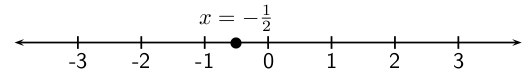
\includegraphics[width=.8\columnwidth]{col11306.imgs/m39254_MG10C10_001.png} % m39254;MG10C10\_001.png;;;6.0;8.5;
\begin{center}
\begin{pspicture}(-4,0.75)(4,1.75)
%\psgrid
\psline[arrows=<->](-4,1)(4,1)
\psdot[dotsize=5pt](-0.5,1)
\multido{\n=-3+1}{7}
{\uput[d](\n,1){\n}
\psline(\n,1.1)(\n,0.9)}
\uput[u](-0.5,1){$x=-\frac{1}{2}$}
\end{pspicture}
\end{center}
      \vspace{2pt}
    \vspace{.1in}
    \end{center}
 \end{figure}       
      \par 
      \label{m39254*id157636}Now let us solve the inequality $2x+2\^{a}‰¤1$.\par 
      \label{m39254*id157661}\nopagebreak\noindent{}
        
    \begin{equation}
    \begin{array}{ccc}\hfill 2x+2& \^{a}‰¤& 1\hfill \\ \hfill 2x& \^{a}‰¤& 1-2\hfill \\ \hfill 2x& \^{a}‰¤& -1\hfill \\ \hfill x& \^{a}‰¤& -\frac{1}{2}\hfill \end{array}\tag{9.57}
      \end{equation}
      \label{m39254*id157764}If we represent this answer on a number line, we get\par 
      \label{m39254*id157770}
    \setcounter{subfigure}{0}
	\begin{figure}[H] % horizontal\label{m39254*id157774}
    \begin{center}
    \label{m39254*id157774!!!underscore!!!media}\label{m39254*id157774!!!underscore!!!printimage}
%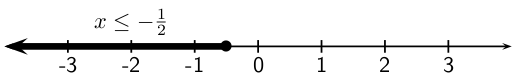
\includegraphics[width=.8\columnwidth]{col11306.imgs/m39254_MG10C10_002.png} % m39254;MG10C10\_002.png;;;6.0;8.5;
\begin{center}
\begin{pspicture}(-4,0.75)(4,1.75)
%\psgrid
\psline[arrows=<->](-4,1)(4,1)
\psdot[dotsize=5pt](-0.5,1)
\multido{\n=-3+1}{7}
{\uput[d](\n,1){\n}
\psline(\n,1.1)(\n,0.9)}
\uput[u](-2,1){$x\le-\frac{1}{2}$}
\psline[linewidth=3pt]{->}(-0.5,1)(-4,1)
\end{pspicture}
\end{center}
      \vspace{2pt}
    \vspace{.1in}
    \end{center}
 \end{figure}       
      \par 
      \label{m39254*id157780}As you can see, for the equation, there is only a single value of $x$ for which the equation is true. However, for the inequality, there is a range of values for which the inequality is true. This is the main difference between an equation and an inequality.\par 
\label{m39254*eip-441}
    \setcounter{subfigure}{0}
	\begin{figure}[H] % horizontal\label{m39254*inequalities-1}
    \textnormal{Khan academy video on inequalities - 1}\vspace{.1in} \nopagebreak
  \label{m39254*yt-media4}\label{m39254*yt-video4}
            \raisebox{-5 pt}{ 
\includegraphics[width=0.5cm]{col11306.imgs/summary_www.png}} { (Video:  MG10074 )}
      \vspace{2pt}
    \vspace{.1in}
 \end{figure}       \par \label{m39254*eip-749}
    \setcounter{subfigure}{0}
	\begin{figure}[H] % horizontal\label{m39254*inequalities-2}
    \textnormal{Khan academy video on inequalities - 2}\vspace{.1in} \nopagebreak
  \label{m39254*yt-media5}\label{m39254*yt-video5}
            \raisebox{-5 pt}{ 
\includegraphics[width=0.5cm]{col11306.imgs/summary_www.png}} { (Video:  MG10075 )}
      \vspace{2pt}
    \vspace{.1in}
 \end{figure}       \par \label{m39254*secfhsst!!!underscore!!!id4213}\vspace{.5cm} 
      \noindent
      \hspace*{-30pt}
\includegraphics[width=0.5in]{col11306.imgs/pspencil2.png}   \raisebox{25mm}{   
      \begin{mdframed}[linewidth=4, leftmargin=40, rightmargin=40]  
      \begin{exercise}
    \noindent\textbf{Exercise 9.11:  Linear Inequalities }
      \label{m39254*probfhsst!!!underscore!!!id4214}
      \label{m39254*id157808}Solve for $r$: $6-r\greatthan{}2$ \par 
      \vspace{5pt}
      \label{m39254*solfhsst!!!underscore!!!id4217}\noindent\textbf{Solution to Exercise } \label{m39254*listfhsst!!!underscore!!!id4217}\begin{enumerate}[noitemsep, label=\textbf{Step} \textbf{\arabic*}. ] 
            \leftskip=20pt\rightskip=\leftskip\item  
      \label{m39254*id157858}\nopagebreak\noindent{}
        
    \begin{equation}
    \begin{array}{cc}\hfill -r\greatthan{}2-6\\ \hfill -r\greatthan{}-4\end{array}\tag{9.58}
      \end{equation}
      \item  
      \label{m39254*id157909}When you multiply by a minus sign, the direction of the inequality changes.\par 
      \label{m39254*id157913}\nopagebreak\noindent{}
        
    \begin{equation}
    r\lessthan{}4\tag{9.59}
      \end{equation}
      \item  
      \label{m39254*id157934}
    \setcounter{subfigure}{0}
	\begin{figure}[H] % horizontal\label{m39254*id157937}
    \begin{center}
    \label{m39254*id157937!!!underscore!!!media}\label{m39254*id157937!!!underscore!!!printimage}
%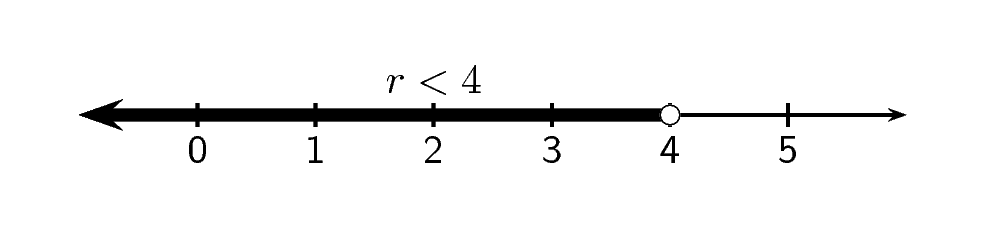
\includegraphics{col11306.imgs/m39254_MG10C10_003.png} % ;MG10C10\_003.png;;;6.0;8.5;
\begin{center}
\begin{pspicture}(-1,0.4)(6,1.6)
%\psgrid
\psline[arrows=<->](-1,1)(6,1)
\multido{\n=0+1}{6}
{\uput[d](\n,1){\n}
\psline(\n,1.1)(\n,0.9)}
\uput[u](2,1){$r<4$}
\psline[linewidth=3pt]{->}(4,1)(-1,1)
\psdot[dotsize=5pt,dotstyle=o](4,1)
\end{pspicture}
\end{center}
}
      \vspace{2pt}
    \vspace{.1in}
    \end{center}
 \end{figure}       
      \par 
      \end{enumerate}
    \end{exercise}
    \end{mdframed}
    }
    \noindent
\label{m39254*secfhsst!!!underscore!!!id4271}\vspace{.5cm} 
      \noindent
      \hspace*{-30pt}
\includegraphics[width=0.5in]{col11306.imgs/pspencil2.png}   \raisebox{25mm}{   
      \begin{mdframed}[linewidth=4, leftmargin=40, rightmargin=40]  
      \begin{exercise}
    \noindent\textbf{Exercise 9.12:  Linear Inequalities }
      \label{m39254*probfhsst!!!underscore!!!id4272}
      \label{m39254*id157972}Solve for $q$: $4q+3\lessthan{}2\left(q+3\right)$ and represent the solution on a number line. \par 
      \vspace{5pt}
      \label{m39254*solfhsst!!!underscore!!!id4275}\noindent\textbf{Solution to Exercise } \label{m39254*listfhsst!!!underscore!!!id4275}\begin{enumerate}[noitemsep, label=\textbf{Step} \textbf{\arabic*}. ] 
            \leftskip=20pt\rightskip=\leftskip\item  
      \label{m39254*id158035}\nopagebreak\noindent{}
        
    \begin{equation}
    \begin{array}{ccc}\hfill 4q+3& \lessthan{}& 2\left(q+3\right)\hfill \\ \hfill 4q+3& \lessthan{}& 2q+6\hfill \end{array}\tag{9.60}
      \end{equation}
      \item  
      \label{m39254*id158117}\nopagebreak\noindent{}
        
    \begin{equation}
    \begin{array}{ccc}\hfill 4q+3& \lessthan{}& 2q+6\hfill \\ \hfill 4q-2q& \lessthan{}& 6-3\hfill \\ \hfill 2q& \lessthan{}& 3\hfill \end{array}\tag{9.61}
      \end{equation}
      \item  
      \label{m39254*id158212}\nopagebreak\noindent{}
    \begin{equation}
    \begin{array}{ccccc}\hfill 2q& \lessthan{}& 3\hfill & \mathrm{Divide\; both\; sides\; by}\phantom{\rule{2pt}{0ex}}2\hfill & \\ \hfill q& \lessthan{}& \frac{3}{2}\hfill & \end{array}\tag{9.62}
      \end{equation}
      \item  
      \label{m39254*id158284}
    \setcounter{subfigure}{0}
	\begin{figure}[H] % horizontal\label{m39254*id158287}
    \begin{center}
    \label{m39254*id158287!!!underscore!!!media}\label{m39254*id158287!!!underscore!!!printimage}
%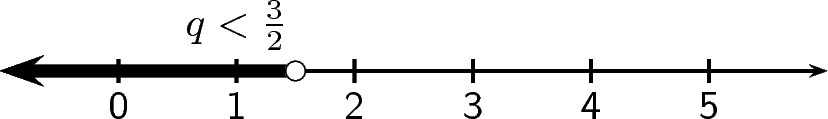
\includegraphics{col11306.imgs/m39254_MG10C10_004.png} % ;MG10C10\_004.png;;;6.0;8.5;
\begin{center}
\begin{pspicture}(-1,0.4)(6,1.6)
%\psgrid
\psline[arrows=<->](-1,1)(6,1)
\multido{\n=0+1}{6}
{\uput[d](\n,1){\n}
\psline(\n,1.1)(\n,0.9)}
\uput[u](1,1){$q<\frac{3}{2}$}
\psline[linewidth=3pt]{->}(1.5,1)(-1,1)
\psdot[dotsize=5pt,dotstyle=o](1.5,1)
\end{pspicture}
\end{center}

      \vspace{2pt}
    \vspace{.1in}
    \end{center}
 \end{figure}       
      \par 
      \end{enumerate}
    \end{exercise}
    \end{mdframed}
    }
    \noindent
\label{m39254*secfhsst!!!underscore!!!id4447}\vspace{.5cm} 
      \noindent
      \hspace*{-30pt}
\includegraphics[width=0.5in]{col11306.imgs/pspencil2.png}   \raisebox{25mm}{   
      \begin{mdframed}[linewidth=4, leftmargin=40, rightmargin=40]  
      \begin{exercise}
    \noindent\textbf{Exercise 9.13:  Compound Linear Inequalities }
      \label{m39254*probfhsst!!!underscore!!!id4448}
      \label{m39254*id158322}Solve for $x$: $5\^{a}‰¤x+3\lessthan{}8$ and represent solution on a number line. \par 
      \vspace{5pt}
      \label{m39254*solfhsst!!!underscore!!!id4451}\noindent\textbf{Solution to Exercise } \label{m39254*listfhsst!!!underscore!!!id4451}\begin{enumerate}[noitemsep, label=\textbf{Step} \textbf{\arabic*}. ] 
            \leftskip=20pt\rightskip=\leftskip\item  
      \label{m39254*id158378}\nopagebreak\noindent{}
        
    \begin{equation}
    \begin{array}{ccc}\hfill 5-3\^{a}‰¤& x+3-3& \lessthan{}8-3\hfill \\ \hfill 2\^{a}‰¤& x& \lessthan{}5\hfill \end{array}\tag{9.63}
      \end{equation}
      \item  
      \label{m39254*id158456}
    \setcounter{subfigure}{0}
	\begin{figure}[H] % horizontal\label{m39254*id158459}
    \begin{center}
    \label{m39254*id158459!!!underscore!!!media}\label{m39254*id158459!!!underscore!!!printimage}
%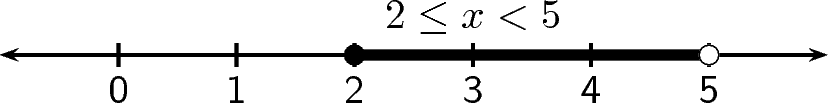
\includegraphics{col11306.imgs/m39254_MG10C10_005.png} % ;MG10C10\_005.png;;;6.0;8.5;
\begin{center}
\begin{pspicture}(-1,0.4)(6,1.6)
%\psgrid
\psline[arrows=<->](-1,1)(6,1)
\multido{\n=0+1}{6}
{\uput[d](\n,1){\n}
\psline(\n,1.1)(\n,0.9)}
\uput[u](3,1){$2\le x < 5$}
\psline[linewidth=2.5pt](2,1)(5,1)
\psdot[dotsize=5pt,dotstyle=o](5,1)
\psdot[dotsize=5pt](2,1)
\end{pspicture}
\end{center}

      \vspace{2pt}
    \vspace{.1in}
    \end{center}
 \end{figure}       
      \par 
      \end{enumerate}
    \end{exercise}
    \end{mdframed}
    }
    \noindent
            \subsection{ Exercise: Linear Inequalities }
            \nopagebreak
      \label{m39254*id158488}\begin{enumerate}[noitemsep, label=\textbf{\arabic*}. ] 
            \label{m39254*uid82}\item Solve for $x$ and represent the solution graphically:
\label{m39254*id158514}\begin{enumerate}[noitemsep, label=\textbf{\alph*}. ] 
            \label{m39254*uid83}\item $3x+4\greatthan{}5x+8$\label{m39254*uid84}\item $3\left(x-1\right)-2\^{a}‰¤6x+4$\label{m39254*uid85}\item $\frac{x-7}{3}\greatthan{}\frac{2x-3}{2}$\label{m39254*uid86}\item $-4\left(x-1\right)\lessthan{}x+2$\label{m39254*uid87}\item $\frac{1}{2}x+\frac{1}{3}\left(x-1\right)\^{a}‰¥\frac{5}{6}x-\frac{1}{3}$\end{enumerate}
        \hspace{1ex}        
\label{m39254*uid88}\item Solve the following inequalities. Illustrate your answer on a number line if $x$ is a real number.
\label{m39254*id158773}\begin{enumerate}[noitemsep, label=\textbf{\alph*}. ] 
            \label{m39254*uid89}\item $-2\^{a}‰¤x-1\lessthan{}3$
\label{m39254*uid90}\item $-5\lessthan{}2x-3\^{a}‰¤7$
\end{enumerate}
\label{m39254*uid91}\item Solve for $x$: $7\left(3x+2\right)-5\left(2x-3\right)\greatthan{}7$\hspace{1ex}Illustrate this answer on a number line.\hspace{1ex}        
\end{enumerate}
\label{m39254**end}
\par \raisebox{-5 pt}{
\includegraphics[width=0.5cm]{col11306.imgs/summary_www.png}} Find the answers with the shortcodes:
 \par \begin{tabular}[h]{cccccc}
 (1.) lcJ  &  (2.) lcS  &  (3.) lch  & \end{tabular}
          \section{ Summary}
    \nopagebreak
            \label{m39263} $ \hspace{-5pt}\begin{array}{cccccccccccc}   \end{array} $ \hspace{2 pt}\raisebox{-5 pt}{\includegraphics[width=0.5cm]{col11306.imgs/summary_www.png}} {(section shortcode: MG10080 )} \par 
% \label{m39263*eip-967}
%             \subsection{ ualitiesualities: Summary and exercises}
%             \nopagebreak
\label{m39263*eip-909}\begin{itemize}[noitemsep]
            \item A linear equation is an
equation where the power of the variable(letter, e.g. $x$) is 1(one). A linear equation has at most one solution\item A quadratic equation is an equation where the power of the variable is at most 2. A quadratic equation has at most two solutions\item Exponential equations generally have the unknown variable as the power. The general form of an exponential equation is: 
	$k{a}^{\left(x+p\right)}=m$\item A linear inequality is similar to a linear equation and has the power of the variable equal to 1.
	When you divide or multiply both sides of an inequality by any number with a minus sign, the direction of the inequality changes. You can solve linear inequalities using the same methods used for linear equations\item When two unknown variables need to be solved for, two equations are required and these equations are known as simultaneous equations. There are two ways to solve linear simultaneous equations: graphical solutions and algebraic solutions. To solve graphically you draw the graph of each equation and the solution will be the co-ordinates of the point of intersection. To solve algebraically you solve equation one, for variable one and then substitute that solution into equation two and solve for variable two.\item Literal equations are equations where you have several letters (variables) and you rearrange the equation to find the solution in terms of one letter (variable)\item Mathematical modelling is where we take a problem and we write a set of equations that represent the problem mathematically. The solution of the equations then gives the solution to the problem.\end{itemize}
        \label{m39263*uid119}
            \section{ End of Chapter Exercises}
            \nopagebreak
        \label{m39263*id162833}\begin{enumerate}[noitemsep, label=\textbf{\arabic*}. ] 
            \label{m39263*uid120}\item What are the roots of the quadratic equation ${x}^{2}-3x+2=0$\hspace{1ex}?
\hspace{1ex}        
\label{m39263*uid121}\item What are the solutions to the equation ${x}^{2}+x=6$\hspace{1ex}?
\hspace{1ex}        
\label{m39263*uid122}\item In the equation $y=2{x}^{2}-5x-18$, which is a value of $x$ when $y=0$\hspace{1ex}?
\hspace{1ex}        
\label{m39263*uid123}\item Manuel has 5 more CDs than Pedro has. Bob has twice as many CDs as Manuel has. Altogether the boys have 63 CDs. Find how many CDs each person has.
\hspace{1ex}        
\label{m39263*uid124}\item Seven-eighths of a certain number is 5 more than one-third of the number. Find the number.
\hspace{1ex}        
\label{m39263*uid125}\item A man runs to a telephone and back in 15 minutes. His speed on the way to the telephone is 5 m/s and his speed on the way back is 4 m/s. Find the distance to the telephone.
\hspace{1ex}        
\label{m39263*uid126}\item Solve the inequality and then answer the questions:
$\frac{x}{3}-14\greatthan{}14-\frac{x}{4}$\label{m39263*id163069}\begin{enumerate}[noitemsep, label=\textbf{\alph*}. ] 
            \label{m39263*uid127}\item If $x\^{a}ˆˆ\mathbb{R}$, write the solution in interval notation.
\label{m39263*uid128}\item if $x\^{a}ˆˆ\mathbb{Z}$ and $x\lessthan{}51$, write the solution as a set of integers.
\end{enumerate}
        \hspace{1ex}        
\label{m39263*uid129}\item Solve for $a$: $\frac{1-a}{2}-\frac{2-a}{3}\greatthan{}1$\hspace{1ex}        
\label{m39263*uid130}\item Solve for $x$: $x-1=\frac{42}{x}$\hspace{1ex}        
\label{m39263*uid131}\item Solve for $x$ and $y$: $7x+3y=13$ and $2x-3y=-4$\hspace{1ex}        
\end{enumerate}
    \label{m39263**end}
  \label{108b030756318cdc732e3f8c9c583cfb**end}
\par \raisebox{-5 pt}{\includegraphics[width=0.5cm]{col11306.imgs/summary_www.png}} Find the answers with the shortcodes:
 \par \begin{tabular}[h]{cccccc}
 (1.) lcG  &  (2.) lc7  &  (3.) lcA  &  (4.) lco  &  (5.) lcs  &  (6.) lcH  &  (7.) lc6  &  (8.) lcF  &  (9.) lcL  &  (10.) lcM  & \end{tabular}
